\documentclass[FCD_GNN.tex]{subfiles}

\begin{document}
\chapter{Experiments}
\label{chapter:Experiments}

This chapter presents the main experimental results, focusing on the influence
of different textual prompts on model performance.
It includes experiments with mixed and incorrect textual descriptions, as well
as an analysis of how the addition of GNN blocks affects the final
segmentation results and the challenges encountered in this setting.

\section{Basic Experiments}
To systematically assess the contribution of each component of the proposed
multimodal architecture, we gradually enable individual decoder modules—
geometry-based upsampling, self-attention, and finally text-conditioned
cross-attention.
This stepwise experimental design allows isolating the effect of textual
guidance and ensures that any improvement in lesion detection quality can be
attributed to a specific architectural modification rather than confounding
changes.

In all configurations, we freeze both encoders: the visual encoder (the
\textbf{MELD} backbone) and the text encoder.
Although \textbf{RadBERT} was used as the initial language model during the early
stages of this work—primarily because it was the first domain-specific model that
integrated smoothly into the pipeline—the choice of text encoder was later
examined more systematically.
After observing that textual signals substantially influence lesion detection
quality, we conducted an additional study comparing several biomedical and
radiology-oriented language models.

These language models differ in the domain and scale of their pretraining data:
\textbf{RadBERT} and \textbf{BlueBERT} are pretrained on radiology reports and
clinical text, while \textbf{PubMedBERT} is trained on large-scale biomedical
literature.
The results of this analysis (see Appendix~\nameref{sec:semantic_analysis})
motivated the inclusion of multiple text-encoder variants in the experimental
evaluation.

Across all variants, the geometry-based upsampling path
(\texttt{HexUnpool} + \texttt{SpiralConv}) and the final segmentation head are
always trained, while both encoders remain frozen
(Figure~\ref{fig:basic_model}).
The experimental variants differ only in (i) whether the \texttt{GuideDecoder}
is inserted before the upsampling path and (ii) the type of atlas-derived
textual input used.
The pretrained \texttt{Vision-only} model (described below) is used to initialize
the decoder for all variants except the MELD-only baseline, which is trained
from scratch.

We consider the following configurations:

\begin{itemize}
    \item \textbf{MELD.} The pretrained \ac{meld} model was evaluated on the test set without any additional training or fine-tuning and is used as the baseline (see Figure~\ref{fig:meld_arch}).

    \item \textbf{Vision--only (Unpool + Spiral, no text).}
    In this configuration, the pretrained \ac{meld} model is used to provide multi--scale visual features extracted from its decoder at each stage.
    The text branch and the self--/cross--attention modules of the \texttt{GuideDecoder} are disabled, while the geometry--based upsampling components are retained (see Figure~\ref{fig:exp1_arch}).
    The decoder features from \ac{meld} are reshaped and passed directly through the upsampling path (\texttt{HexUnpool} + \texttt{SpiralConv}) and then to the segmentation head.
    No textual input is used in this variant, so the prediction relies solely on image--derived features.

    \begin{figure}[H]
        \centering
        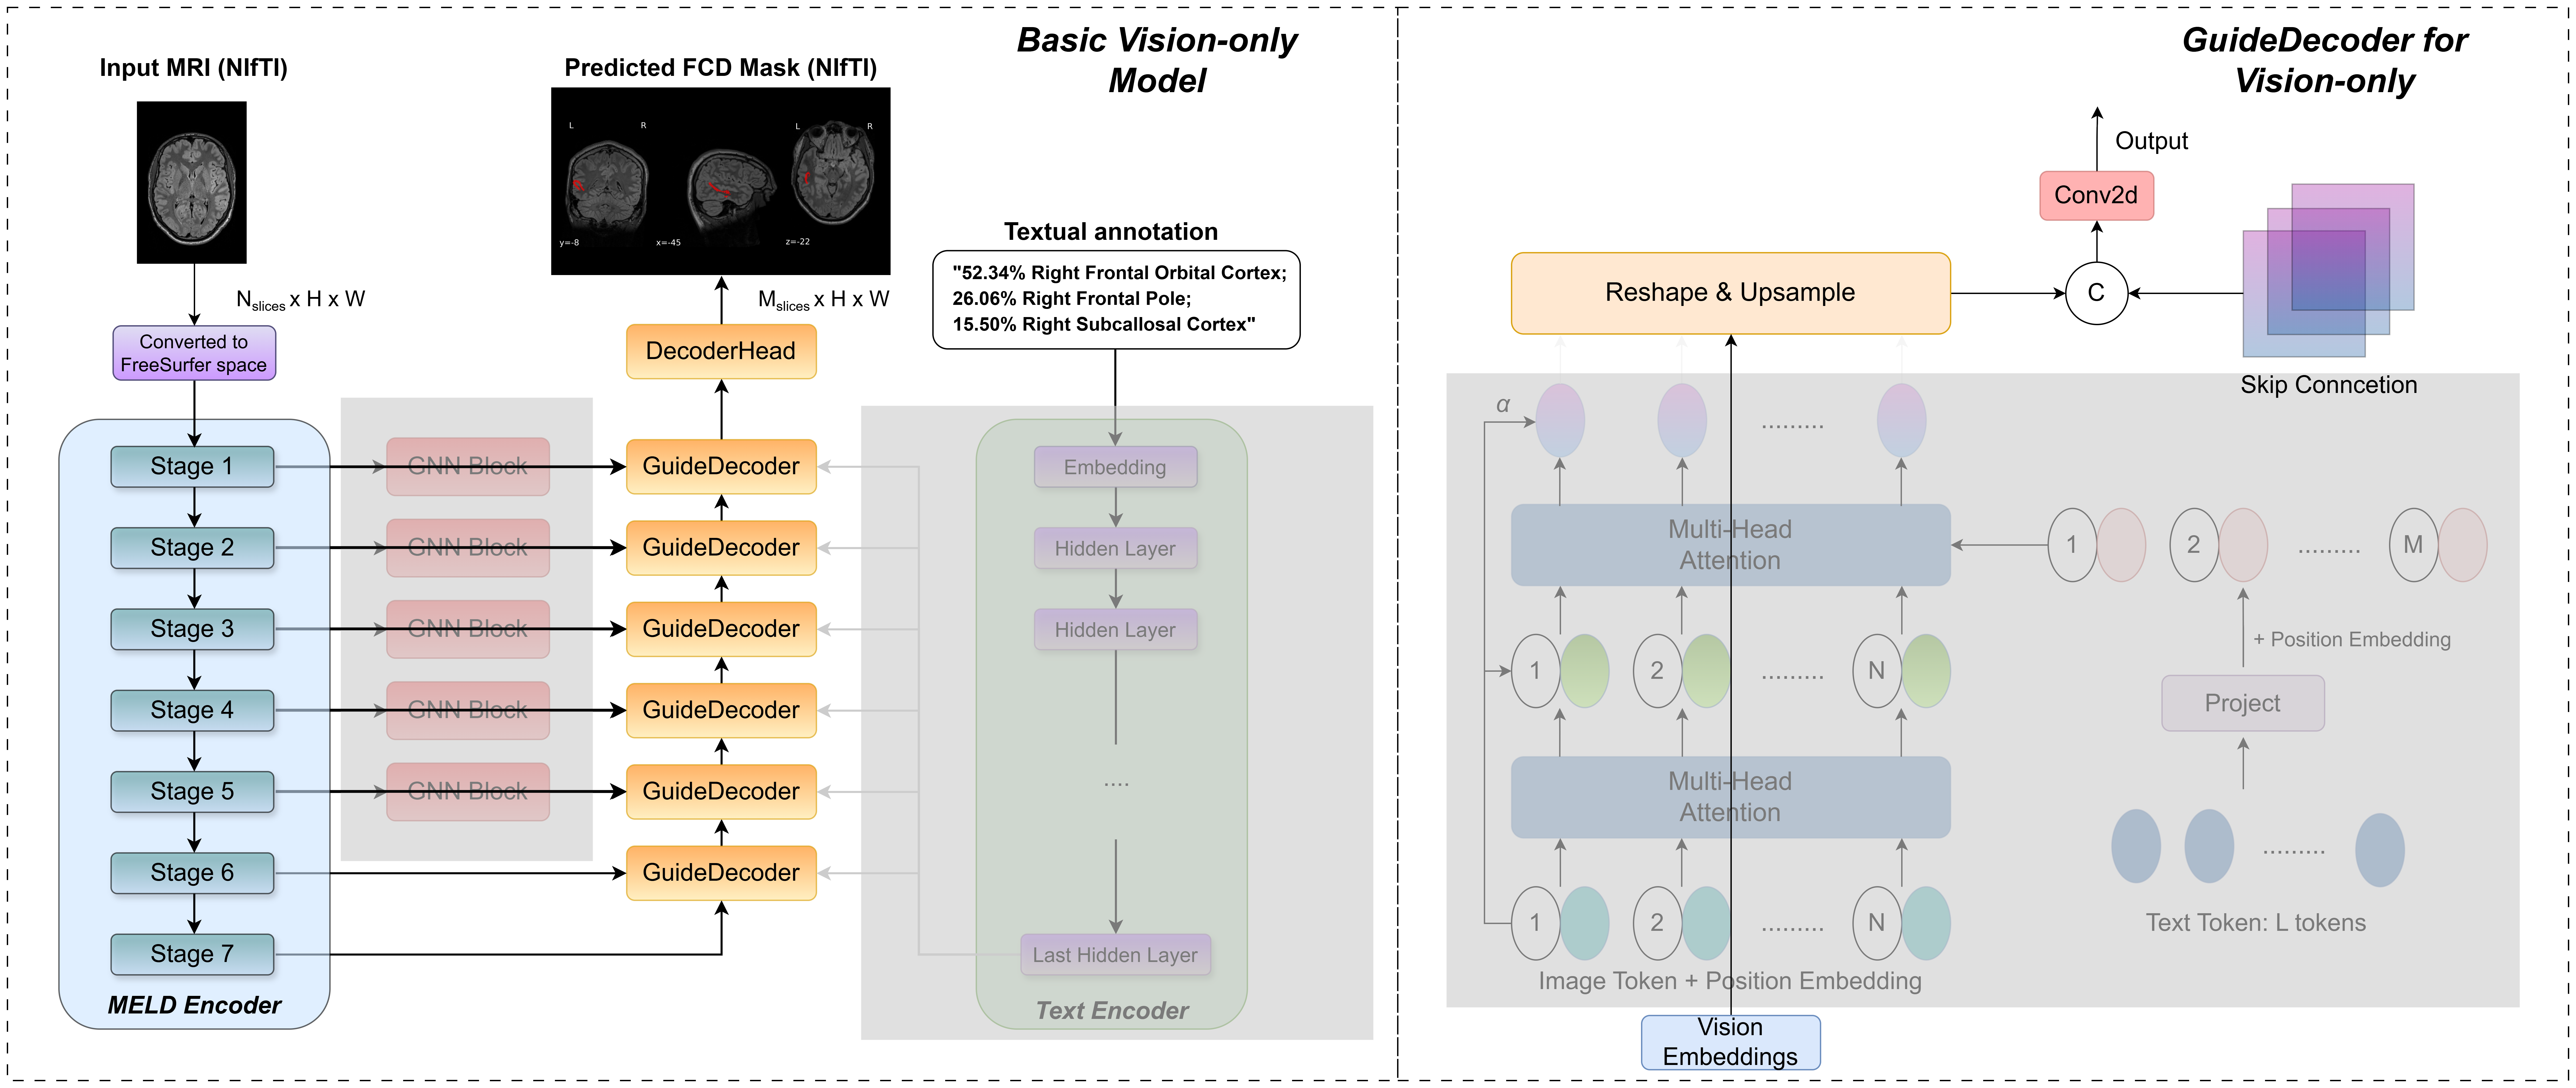
\includegraphics[width=\textwidth]{pictures/BasicModelExp1.png}
        \caption{Architecture of Vision--only: the text branch and the self-/cross-attention modules in the \texttt{GuideDecoder} are disabled, and MELD vision features are fed directly into the geometry-based upsampling path and segmentation head.}
        \label{fig:exp1_arch}
    \end{figure}

    \item \textbf{Vision--only+SA (GuideDecoder: self-attention only).}
    As in \texttt{Vision--only}, multi--scale visual features are extracted from the pretrained \ac{meld} decoder and used as input to the \texttt{GuideDecoder}.
    One \texttt{GuideDecoder} block is inserted at each decoder level (D6--D1), i.e., one block per upsampling stage, to refine the features using self--attention before the subsequent upsampling step (see Figure~\ref{fig:exp2_arch}).
    The text branch remains disabled; therefore, cross--attention is not applied and each \texttt{GuideDecoder} performs self--attention only.
    The upsampling path and segmentation head are kept identical to \texttt{Vision--only}.

    \begin{figure}[H]
        \centering
        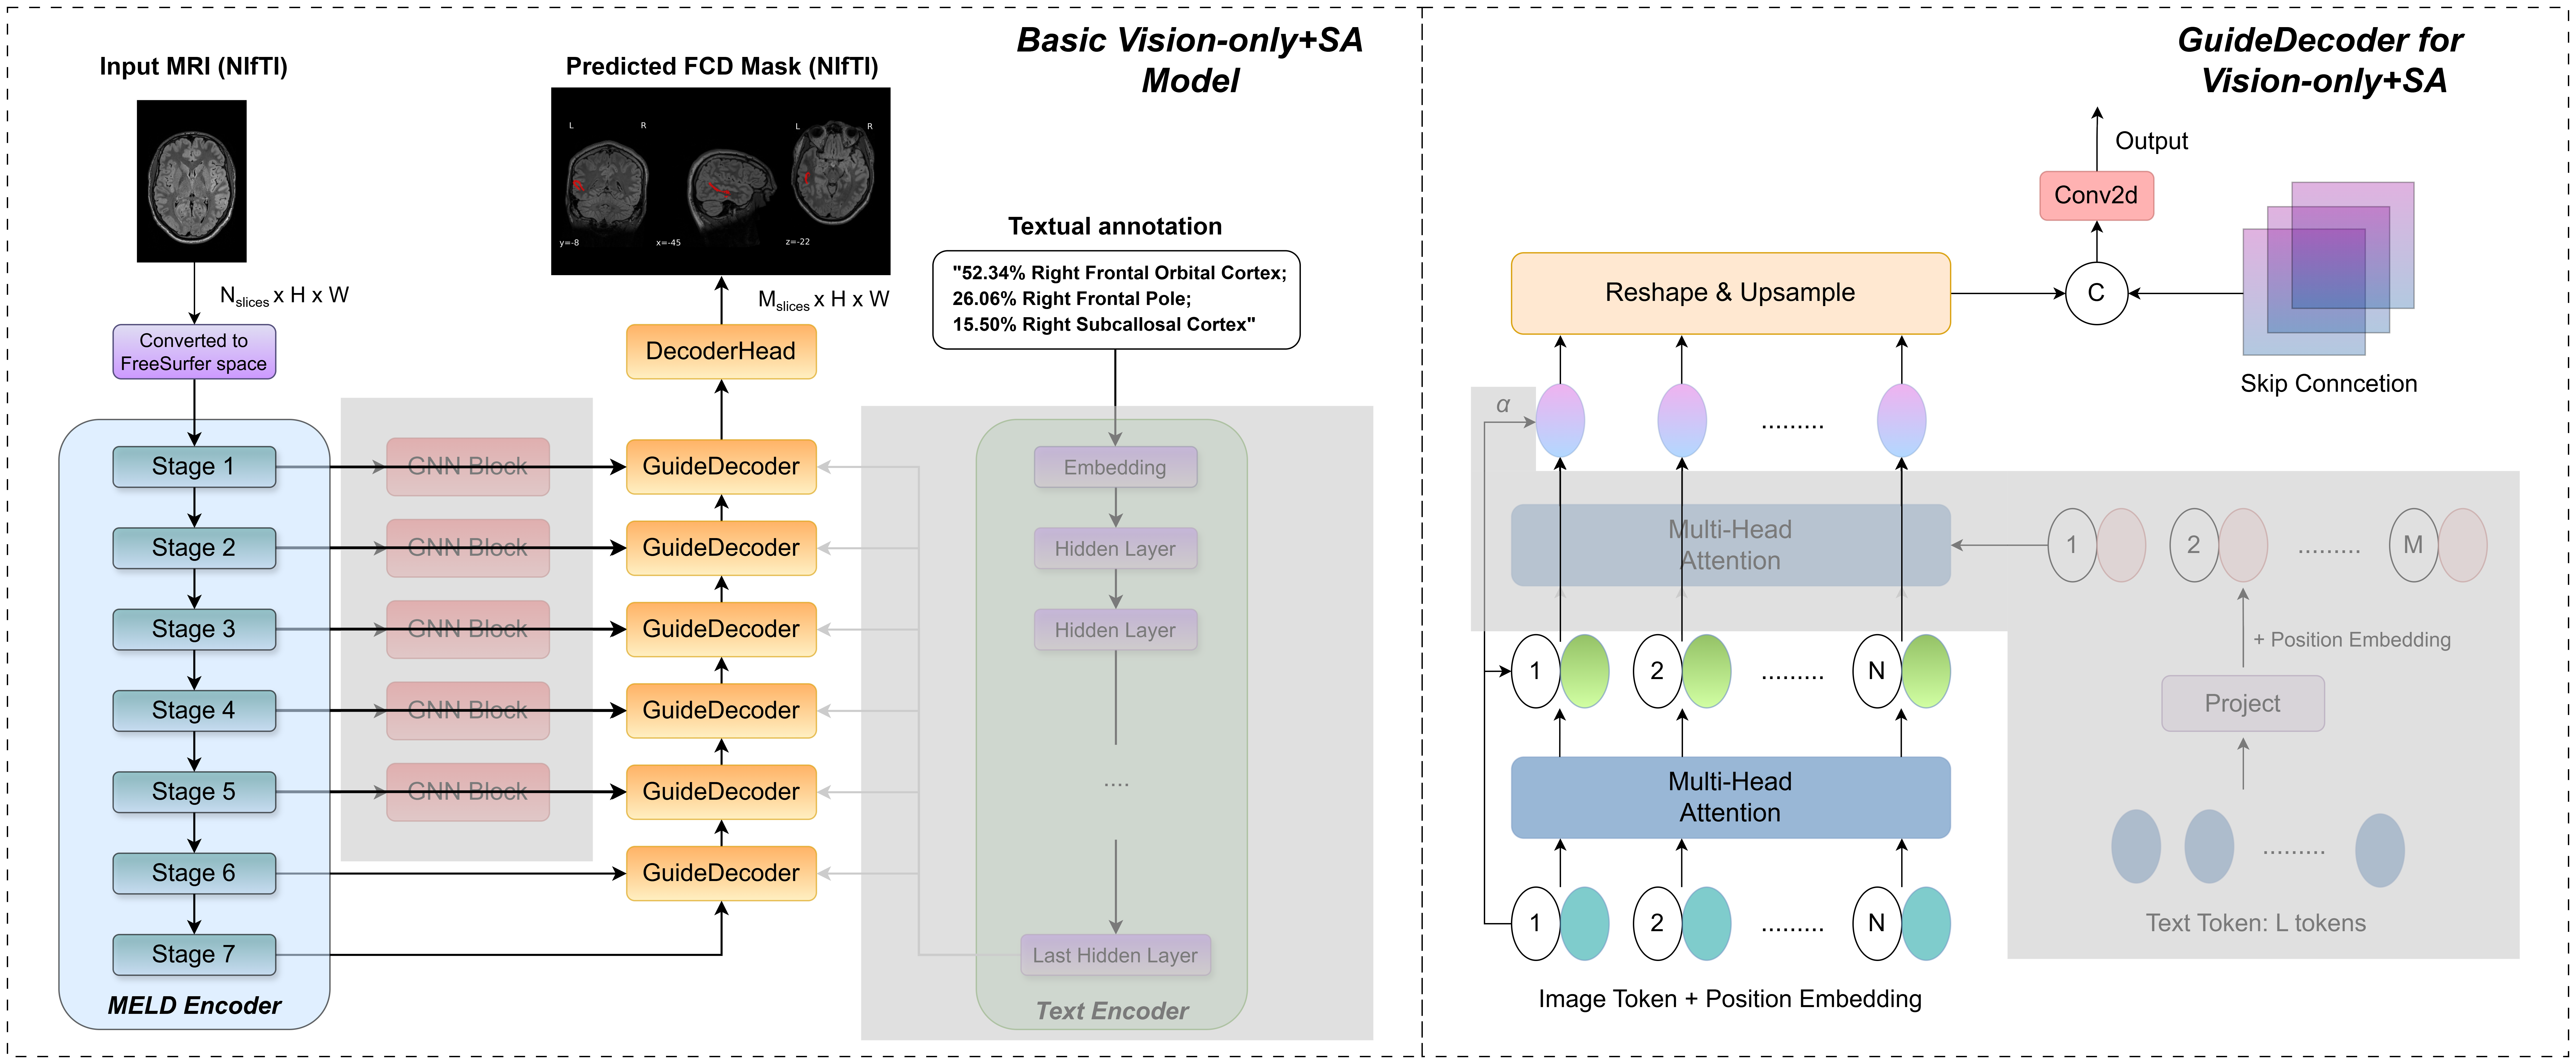
\includegraphics[width=\textwidth]{pictures/BasicModelExp2.png}
        \caption{Architecture of \texttt{Vision--only+SA}: each \texttt{GuideDecoder} block contains a self-attention head, while the text branch remains disabled.}
        \label{fig:exp2_arch}
    \end{figure}
    
    \item \textbf{Vision+LM (GuideDecoder + Text).}
    As in \texttt{Vision--only} and \texttt{Vision--only+SA}, multi--scale visual features are extracted from the pretrained \ac{meld} decoder and used as input to the \texttt{GuideDecoder}.
    In contrast to \texttt{Vision--only+SA}, the full \texttt{GuideDecoder} is enabled, i.e., self--attention on image tokens and cross--attention between image and text embeddings are applied (see Figure~\ref{fig:basic_model}).
    The only difference across variants is the textual conditioning (Table~\ref{tab:text_variants}):
    % For healthy subjects (no lesion present), the textual input is set to \textit{``No lesion detected.''}

    % \begin{itemize}
    %     \item \emph{full} (complete Atlas annotations): \textit{48.86\% Left Middle Frontal Gyrus; 30.63\% Left Precentral Gyrus; 20.51\% Left Superior Frontal Gyrus}
    % \item \emph{hemi} (hemisphere only): \textit{Left Hemisphere} ; 
    % \item \emph{lobe\_regions} (lobe regions only): \textit{Left Middle Frontal Gyrus; Precentral Gyrus; Superior Frontal Gyrus};
    % % \emph{lobe} (general lobe name only),
    % \item \emph{hemi+lobe\_regions} (hemisphere + lobe regions): \textit{Left Hemisphere; Middle Frontal Gyrus; Precentral Gyrus; Superior Frontal Gyrus} ;
    % \item \emph{hemi+lobe} (hemisphere + lobe): \textit{Left Hemisphere; Frontal lobe}.
    % \end{itemize}


    \begin{figure}[H]
        \centering
        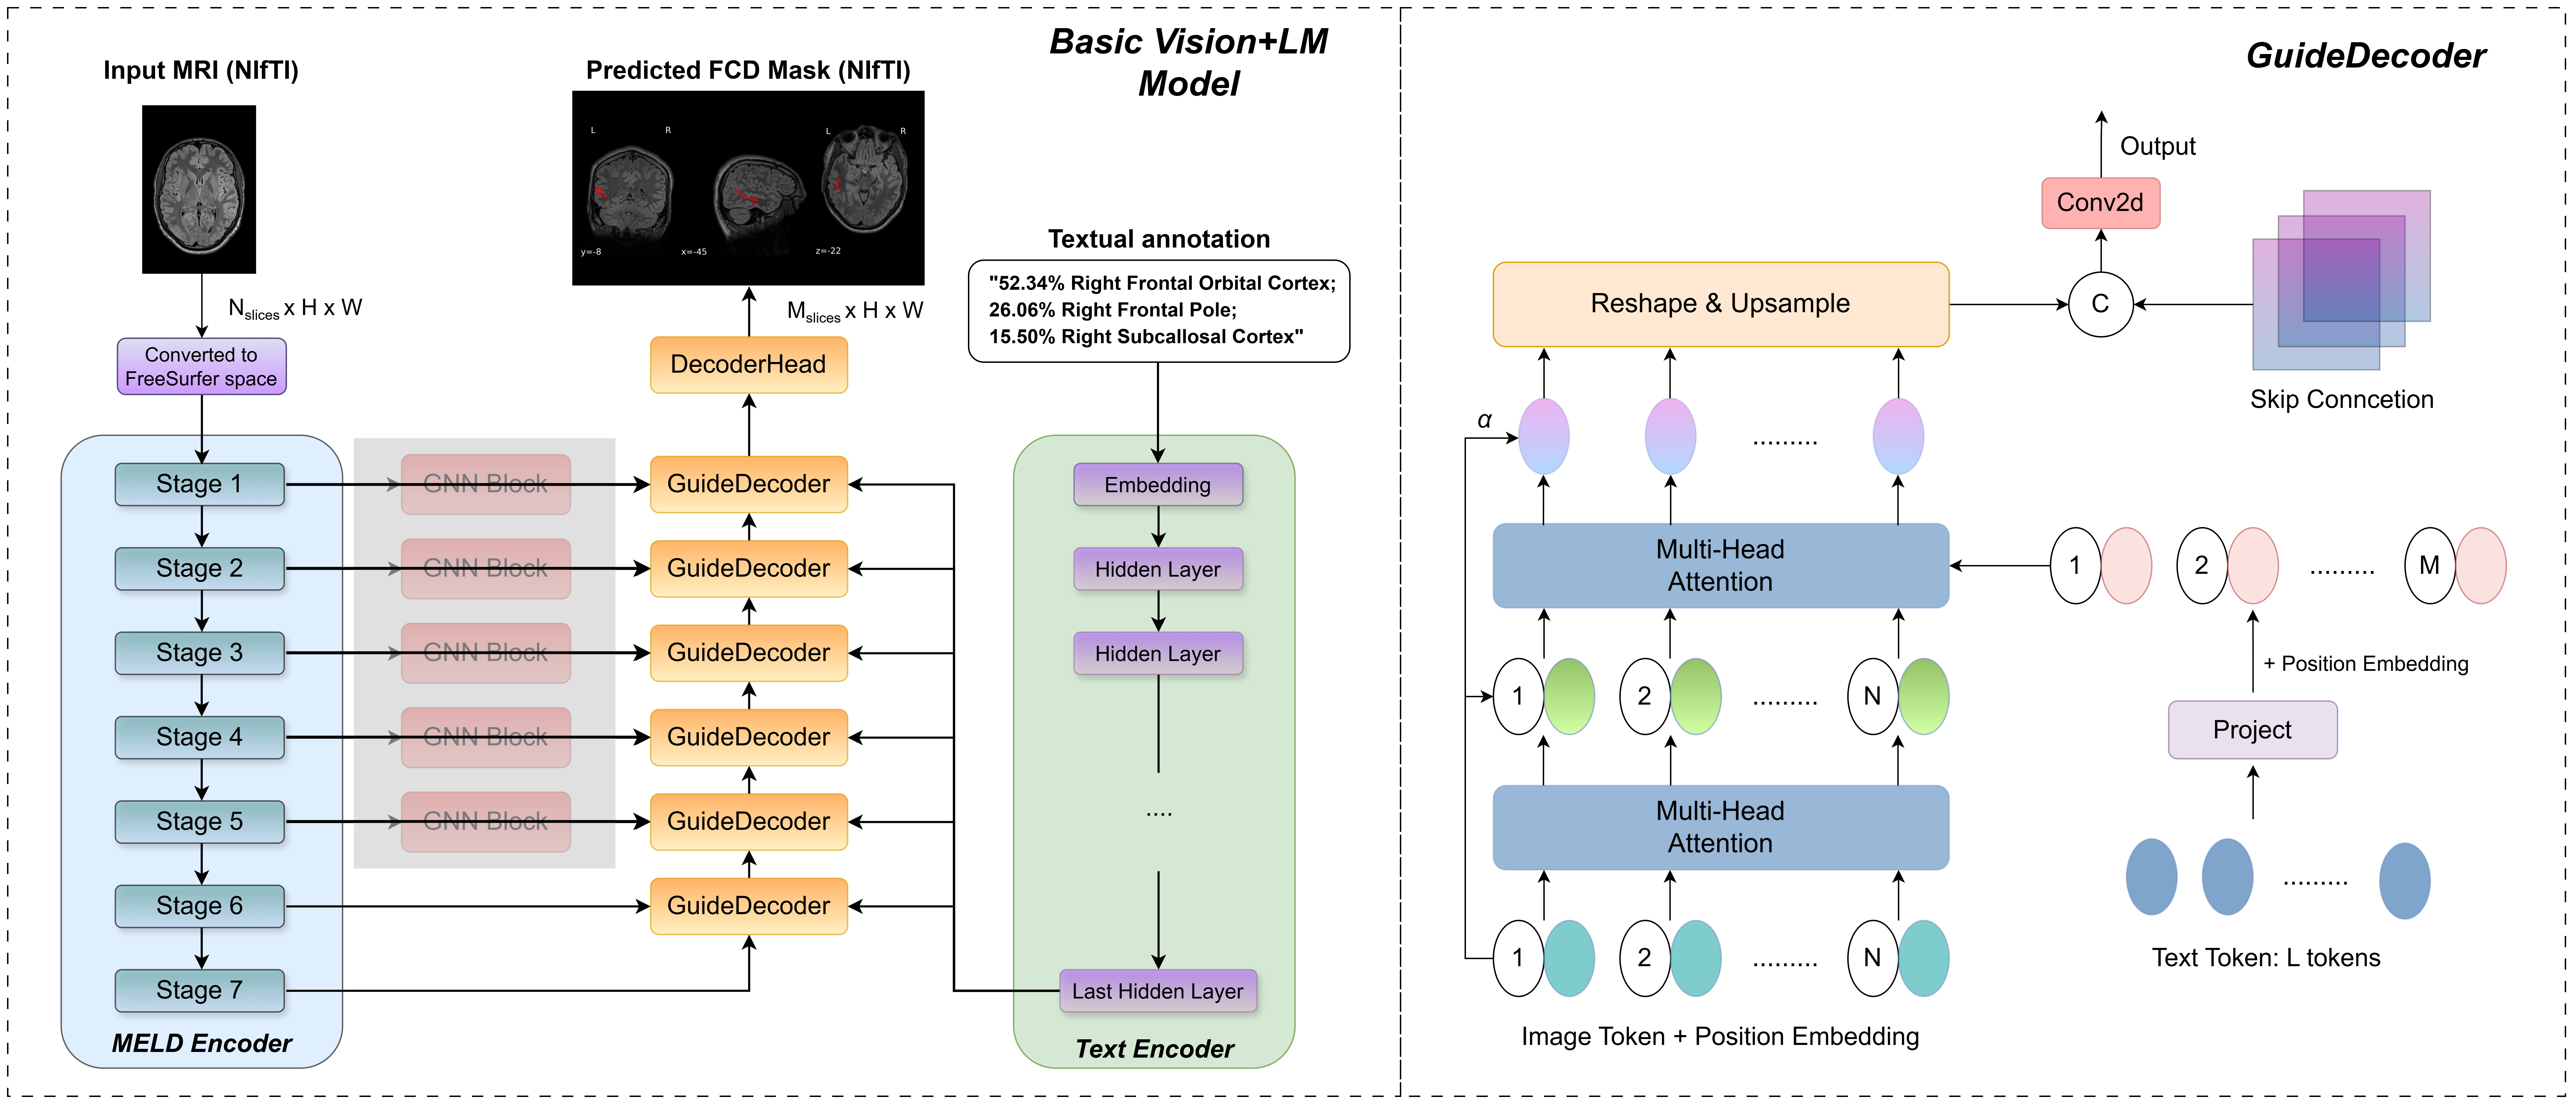
\includegraphics[width=\textwidth]{pictures/BasicModelExp3.png}
        \caption{Architecture of \texttt{Vision+LM}: the full \texttt{GuideDecoder} is used, incorporating both self-attention on visual tokens and cross-attention between visual features and text embeddings.}
        \label{fig:basic_model}
    \end{figure}

    \item \textbf{Vision+LM\_mixed (GuideDecoder + Mixed Text).} 
    Same as \textbf{Vision+LM}, but Atlas descriptions were randomly sampled from the text conditioning variants listed in Table~\ref{tab:text_variants}.

    For each subject, a full Atlas--based description was generated once and all partial textual variants were derived from it.
    During training, one textual variant was randomly sampled independently for each sample at every data loading step.
    Consequently, the same subject could be paired with different textual inputs across epochs.

\end{itemize}

\subsection*{Main cohort}

Table~\ref{tab:main_cohort} presents the median performance on the \ac{meld} test set (main cohort).
In the RadBERT group, defined as all variants using the default RadBERT language encoder 
(without alternative LMs such as BlueBERT or PubMedBERT), the prompt combining 
\textit{hemisphere and lobe-region} terms detected the most lesions, though with only slightly higher Dice, PPV$_\text{pixels}$, and IoU.
Across all models, the PubMedBERT variant achieved the highest number of detected lesions, likely due 
to better domain-context understanding (see Table~\ref{tab:cosine_similarity_models} in the Appendix). 
This clearly demonstrates that selecting an appropriate language model can materially improve 
performance, underscoring the substantial impact of the language encoder.

\begin{table}[ht]
    \tiny
    \centering
    \begin{threeparttable}
    \caption{Median performance on the main cohort (with 95\% confidence intervals).}
    \label{tab:main_cohort}
    \begin{tabular}{lccccccc}
    \textbf{Model} &
    \textbf{Dice} &
    \makecell{\textbf{PPV}\\\textbf{pixels}} &
    \makecell{\textbf{(mean)} \\\textbf{PPV} \\\textbf{clusters}} & \makecell{\textbf{(median)} \\\textbf{PPV} \\\textbf{clusters}} & 
    \textbf{IoU} & 
    \textbf{\makecell{Specificity, \% \\ (N = 193)}} &
    \textbf{\makecell{Sensitivity, \% \\ (N = 259)}} \\
    \midrule
    MELD &
    \makecell{0.230\\(0.107--0.320)} &
    \makecell{0.166\\(0.086--0.220)} &
    \colorbox{green!15}{0.515} &
    \makecell{1.000 \\ (1.000-1.000)} &
    \makecell{0.130\\(0.057--0.190)} &
    \makecell{58.0 (n=112) \\ (51.3--64.8)}&
    \makecell{65.6 (n=170) \\ (59.8--71.4)} \\
    \hline
    Vision--only &
    \makecell{0.238\\(0.125--0.313)} &
    \makecell{0.198\\(0.130--0.318)} &
    0.361 &
    \makecell{1.000 \\ (0.500-1.000)} &
    \makecell{0.135\\(0.066--0.186)} &
    \makecell{31.1 (n=60) \\ (24.9--37.8)} &
    \makecell{69.1 (n=179) \\ (63.3--74.9)} \\
    \hline
    Vision--only+SA &
    \makecell{\colorbox{cyan!15}{0.256} \\ (0.125--0.326)} &
    \makecell{0.204\\ (0.122--0.322)} &
    0.333 &
    \makecell{1.000 \\ (0.500-1.000)} &
    \makecell{\colorbox{cyan!15}{0.147}\\ (0.067--0.195)} &
    \makecell{24.9 (n=48) \\ (19.2--31.1)} &
    \makecell{70.7 (n=183) \\ (65.3--76.1)} \\
    \hline
    Vision+LM: hemi &
    \makecell{0.231\\(0.148--0.285)} &
    \makecell{0.188\\(0.131--0.298)} &
    \colorbox{cyan!15}{0.483} &
    \makecell{0.667 \\ (0.500-1.000)} &
    \makecell{0.131\\(0.080--0.166)} &
    \makecell{\colorbox{green!15}{100.0 (n=193)} \\ (100.0--100.0)} &
    \makecell{71.0 (n=184) \\ (65.6--76.4)} \\
    \hline
    Vision+LM: lobe\_regions &
    \makecell{\colorbox{orange!15}{0.254}\\(0.159--0.332)} &
    \makecell{0.231\\(0.168--0.320)} &
    0.404 &
    \makecell{0.667 \\ (0.500-1.000)} &
    \makecell{\colorbox{orange!15}{0.145}\\(0.086--0.199)} &
    \makecell{\colorbox{green!15}{100.0 (n=193)} \\ (100.0--100.0)} &
    \makecell{\colorbox{orange!15}{72.6 (n=188)} \\ (67.2--78.0)} \\
    \hline
    Vision+LM: \makecell{hemi +\\ lobe\_regions} &
    \makecell{\colorbox{green!15}{0.264}\\(0.180--0.342)} &
    \makecell{\colorbox{orange!15}{0.238}\\(0.160--0.327)} &
    0.333 &
    \makecell{0.500 \\ (0.500-1.000)} &
    \makecell{\colorbox{green!15}{0.152}\\(0.099--0.206)} &
    \makecell{\colorbox{cyan!15}{99.5 (n=192)} \\ (98.4--100.0)} & 
    \makecell{\colorbox{cyan!15}{74.5 (n=193)} \\ (69.1--79.9) } \\
    \hline
    Vision+LM: hemi + lobe &
    \makecell{0.239\\(0.113--0.302)} &
    \makecell{\colorbox{cyan!15}{0.242}\\(0.166--0.353)} &
    0.456 &
    \makecell{0.667 \\ (0.500-1.000)} &
    \makecell{0.136\\(0.060--0.178)} &
    \makecell{\colorbox{cyan!15}{99.5 (n=192)} \\ (98.4--100.0)} & 
    \makecell{71.4 (n=185) \\ (66.0--76.8)} \\
    \hline
    Vision+LM: \makecell{hemi + lobe + \\ BlueBERT} &
    \makecell{0.230\\(0.125--0.305)} &
    \makecell{0.231\\(0.146--0.330)} &
    0.443 &
    \makecell{0.667 \\ (0.500-1.000)} &
    \makecell{0.130\\(0.067--0.180)} &
    \makecell{\colorbox{orange!15}{99.0 (n=191)} \\ (97.4--100.0)} &
    \makecell{71.8 (n=186) \\ (66.4--77.2)} \\
    \hline
    Vision+LM: \makecell{hemi + lobe + \\ PubmedBERT} &
    \makecell{0.233\\(0.139--0.330)} &
    \makecell{\colorbox{cyan!15}{0.242}\\(0.153--0.342)} &
    0.334 &
    \makecell{0.500 \\ (0.500-0.667)} &
    \makecell{0.132\\(0.074--0.198)} &
    \makecell{\colorbox{green!15}{100.0 (n=193)} \\ (100.0--100.0)} &
    \makecell{\colorbox{green!15}{76.4 (n=198)} \\ (71.4--81.5)} \\
    \hline
    Vision+LM: full\_desc &
    \makecell{0.246\\(0.145--0.330)} &
    \makecell{\colorbox{green!15}{0.259}\\(0.178--0.360)} &
    \colorbox{orange!15}{0.478} &
    \makecell{0.667 \\ (0.500-1.000)} &
    \makecell{0.141\\(0.078--0.197)} &
    \makecell{94.3 (n=182) \\ (90.7--97.4)} &
    \makecell{\colorbox{orange!15}{72.6 (n=188)} \\ (67.2--78.0)} \\
    
    \bottomrule
    \end{tabular}
    
    \begin{tablenotes}[flushleft]
    \footnotesize
    \item \textit{Note.} Colors denote rank within each column:
    \colorbox{green!15}{best}, \colorbox{cyan!15}{second}, \colorbox{orange!15}{third}.
    \item \textit{Metrics: } Dice, IoU, PPV$_{\text{pixels}}$, and PPV$_{\text{clusters}}$ are computed on patients only (N = 259). 
    Sensitivity is reported for patients (N = 259), whereas specificity is reported for healthy controls (N = 193).
    \item \textit{Vision+LM prompt variants:}
    \texttt{hemi} -- hemisphere prompt;
    \texttt{lobe\_regions} -- lobe--region prompt;
    \texttt{hemi+lobe} -- hemisphere + coarse lobe prompt;
    \texttt{hemi+lobe+BlueBERT} -- same as previous but with BlueBERT instead of RadBERT; 
    \texttt{hemi+lobe\_regions} -- hemisphere + lobe--region prompt;
    \texttt{full\_desc} -- full atlas prompt.
    \item \textbf{Vision--only} and \textbf{Vision--only+SA} are ablation baselines.
    \end{tablenotes}
    
    \end{threeparttable}
    
\end{table}

In real-world settings, detailed subregion information may be unavailable. 
We therefore evaluated prompts with only general \textit{lobe} names (e.g., \textit{Frontal lobe}, \textit{Temporal lobe}, \textit{Insular lobe}). 
For the RadBERT-based models, performance was very close to the \textit{hemi + lobe\_regions} setup: Dice decreased by $\sim$2.5 \ac{p.p.}, PPV\_{pixels} by $\sim$0.4 \ac{p.p.}, IoU by $\sim$1.6 \ac{p.p.}, and only \textbf{8} fewer lesions were detected. 
Likewise, using only \textit{hemi} descriptions yielded results close to \textit{hemi + lobe}, indicating that even a minimal textual prompt can help identify additional lesion regions.

Also, when using the full textual description (e.g., ``52.34\% Right Frontal Orbital Cortex; 26.06\% Right Frontal Pole; 15.50\% Right Subcallosal Cortex''), the model performed worse than \texttt{hemi+lobe\_regions}.
One possible reason is that the full description contains additional numeric details that may be less informative for the segmentation task, for instance due to overlapping region assignments (the same lesion area contributing to multiple atlas regions).
Since RadBERT was trained on radiology reports, it may not benefit from such highly structured percentage--based inputs.
For comparison, we also tested PubMedBERT, which was trained on a larger biomedical corpus.
Although its Dice, PPV and IoU scores were slightly lower than those of the \texttt{hemi+lobe} configuration with RadBERT, it nevertheless detected \textbf{13 additional lesion clusters}.

We also report specificity, defined as the proportion of healthy controls with no predicted lesion clusters.
Across all \textit{Vision+LM models}, specificity was higher than that of MELD by $\sim$36--42 \ac{p.p.}.
This indicates that the text--conditioned models distinguish healthy from non--healthy cases substantially better.

Throughout this chapter, we do not focus on the median PPV$_{\text{clusters}}$, which is the primary metric reported in the original MELD study.
As shown in Table~\ref{tab:main_cohort}, the median PPV$_{\text{clusters}}$ attains high values across many configurations (often reaching 0.667, with overlapping confidence intervals), providing limited discrimination between models.
In contrast, the mean PPV$_{\text{clusters}}$ exhibits more variation across configurations and is therefore more informative for comparing the methods in our setting.
MELD achieves the highest mean PPV$_{\text{clusters}}$ on the main cohort, with a small margin of $\sim$2--3 \ac{p.p.} over the next two models and a much larger gap to the remaining ones.
On the independent cohort (Table~\ref{tab:independent_cohort}), however, the situation is reversed: the proposed architecture shows improvements of 2--8 \ac{p.p.} compared with the two best-performing baselines.
Overall, the mean PPV$_{\text{clusters}}$ reflects model differences more reliably in our experiments.
For these reasons, in the following experiments we report only the mean PPV$_{\text{clusters}}$, as it allows us to distinguish between models in this study, whereas the median version does not.

\subsection*{Independent cohort}
\begin{table}[H]
    \tiny
    \begin{threeparttable}
    \centering
    \caption{Median performance on the independent cohort (with 95\% confidence intervals).} 
    \label{tab:independent_cohort}
    \begin{tabular}{lccccccc}
    \textbf{Model} &
    \textbf{Dice} &
    \makecell{\textbf{PPV}\\\textbf{pixels}} &
    \makecell{\textbf{(mean)} \\\textbf{PPV}\\\textbf{clusters}} & \makecell{\textbf{(median)}\\\textbf{PPV}\\\textbf{clusters}} & 
    \textbf{IoU} & 
    \textbf{\makecell{Specificity, \% \\ (N = 83)}} &
    \textbf{\makecell{Sensitivity, \% \\ (N = 82)}} \\
    \midrule
    MELD &
    \makecell{0.358\\(0.209--0.465)} &
    \makecell{0.261\\(0.142--0.428)} &
    \colorbox{orange!15}{0.464} &
    \makecell{1.000\\(1.000--1.000)} &
    \makecell{0.218\\(0.117--0.303)} &
    \makecell{55.4 (n=46) \\ (44.6--66.3)} & 
    \makecell{69.5 (n=57) \\ (59.8--79.3)} \\
    \hline
    Vision--only &
    \makecell{\colorbox{cyan!15}{0.376}\\(0.238--0.529)} &
    \makecell{0.443\\(0.243--0.619)} &
    0.350 &
    \makecell{1.000\\(1.000--1.000)} &
    \makecell{\colorbox{cyan!15}{0.232}\\(0.138--0.359)} &
    \makecell{39.8 (n=33) \\ (28.9--50.6)} &
    \makecell{73.2 (n=60) \\ (63.4--82.9)} \\
    \hline
    Vision--only+SA  &
    \makecell{0.342\\ (0.155--0.494)} &
    \makecell{0.381\\ (0.177--0.651)} &
    0.379 &
    \makecell{1.000\\(0.667--1.000)} &
    \makecell{0.206\\ (0.084--0.328)} &
    \makecell{37.3 (n=31) \\ (27.7--48.2)} &
    \makecell{69.5 (n=57) \\ (59.8--79.3)} \\
    \hline
    Vision+LM: hemi  &
    \makecell{0.372\\(0.261--0.515)} &
    \makecell{0.380\\(0.181--0.601)} &
    \colorbox{cyan!15}{0.468} &
    \makecell{1.000\\(1.000--1.000)} &
    \makecell{0.228\\(0.150--0.347)} &
    \makecell{\colorbox{green!15}{100.0 (n=83)} \\ (100.0--100.0)} &
    \makecell{74.4 (n=61) \\ (64.6--84.1)} \\
    \hline
    Vision+LM: lobe\_regions  &
    \makecell{\colorbox{orange!15}{0.373}\\(0.283--0.507)} &
    \makecell{0.407\\(0.233--0.589)} &
    0.257 &
    \makecell{1.000\\(0.667--1.000)} &
    \makecell{\colorbox{orange!15}{0.229}\\(0.165--0.340)} &
    \makecell{\colorbox{green!15}{100.0 (n=83)} \\ (100.0--100.0)} &
    \makecell{\colorbox{cyan!15}{78.0 (n=64)} \\ (68.3--86.6)} \\
    \hline
    Vision+LM: \makecell{hemi+\\lobe\_regions}  &
    \makecell{0.363\\(0.190--0.513)} &
    \makecell{0.434\\(0.209--0.657)} &
    0.359 &
    \makecell{1.000\\(0.500--1.000)} &
    \makecell{0.222\\(0.105--0.345)} &
    \makecell{\colorbox{orange!15}{97.6 (n=81)} \\ (94.0--100.0)} &
    \makecell{74.4 (n=61) \\ (64.6--84.1)} \\
    \hline
    Vision+LM: hemi+lobe  &
    \makecell{0.327\\(0.164--0.512)} &
    \makecell{0.411\\(0.236--0.667)} &
    \colorbox{green!15}{0.545} &
    \makecell{1.000\\(0.667--1.000)} &
    \makecell{0.196\\(0.090--0.344)} &
    \makecell{\colorbox{cyan!15}{98.8 (n=82)} \\ (96.4--100.0)} &
    \makecell{72.0 (n=59) \\ (62.2--81.7)} \\
    \hline
    Vision+LM: \makecell{hemi+lobe+\\BlueBERT} &
    \makecell{0.362\\(0.260--0.498)} &
    \makecell{\colorbox{cyan!15}{0.469}\\(0.267--0.620)} &
    0.356 &
    \makecell{1.000\\(0.750--1.000)} &
    \makecell{0.221\\(0.150--0.331)} &
    \makecell{96.4 (n=80) \\ (91.6--100.0)} &
    \makecell{\colorbox{orange!15}{76.8 (n=63)} \\ (67.1--85.4)} \\
    \hline
    Vision+LM: \makecell{hemi+lobe+ \\ PubmedBERT} &
    \makecell{0.347\\(0.195--0.529)} &
    \makecell{\colorbox{orange!15}{0.457}\\(0.202--0.730)} &
    0.258 &
    \makecell{1.000 \\ (0.500--1.000)} &
    \makecell{0.210\\(0.109--0.360)} &
    \makecell{\colorbox{green!15}{100.0 (n=83)} \\ (100.0--100.0)} &
    \makecell{\colorbox{green!15}{80.5 (n=66)} \\ (72.0--89.0)} \\
    \hline
    Vision+LM: full\_desc  &
    \makecell{\colorbox{green!15}{0.423}\\(0.267--0.506)} &
    \makecell{\colorbox{green!15}{0.484}\\(0.315-0.693)} &
    0.460 &
    \makecell{1.000 \\ (1.000--1.000)} &
    \makecell{\colorbox{green!15}{0.268}\\(0.154-0.339)} &
    \makecell{90.4 (n=75) \\ (83.1--96.4)} &
    \makecell{73.2 (n=60) \\ (63.4--82.9)} \\
    
    \bottomrule
    \end{tabular}
    
    \begin{tablenotes}[flushleft]
    \footnotesize
    \item \textit{Note.} Colors denote rank within each column:
    \colorbox{green!15}{best}, \colorbox{cyan!15}{second}, \colorbox{orange!15}{third}.
    \item \textit{Metrics: } Dice, IoU, PPV$_{\text{pixels}}$, and PPV$_{\text{clusters}}$ are computed on patients only (N = 82). 
    Sensitivity is reported for patients (N = 82), whereas specificity is reported for healthy controls (N = 83).
    \item \textit{Vision+LM prompt variants:}
    \texttt{hemi} -- hemisphere prompt;
    \texttt{lobe\_regions} -- lobe--region prompt;
    \texttt{hemi+lobe} -- hemisphere + coarse lobe prompt;
    \texttt{hemi+lobe+BlueBERT} -- same as previous but with BlueBERT instead of RadBERT; 
    \texttt{hemi+lobe\_regions} -- hemisphere + lobe--region prompt;
    \texttt{full\_desc} -- full atlas prompt.
    \item \textbf{Vision--only} and \textbf{Vision--only+SA} are ablation baselines.
    \end{tablenotes}
    \end{threeparttable}
    
\end{table}
Following the MELD paper, the Bonn cohort is used as an independent test set to assess out-of-distribution generalization.

The models that detected the largest number of lesion clusters were those trained with
\textit{lobe\_regions} prompts in the RadBERT group, as well as the
\textit{hemi + lobe + PubMedBERT} variant across all architectures.
Within the \textit{hemi + lobe} configuration, replacing BlueBERT with PubMedBERT led
to increased lesion detection sensitivity (80.5\% vs.\ 76.8\%).
This gain, however, was accompanied by slightly lower segmentation quality compared to
the BlueBERT-based variant, as reflected by small decreases in Dice (–1.5~p.p.),
PPV$_{\text{pixels}}$ (–1.2~p.p.), and IoU (–1.1~p.p.).
This trade-off is consistent with PubMedBERT’s pretraining on a substantially larger
corpus of biomedical and brain-related clinical text, which enhances its ability to
recognize lesion-related terminology but does not necessarily improve spatial localization.
Overall, the \textit{hemi + lobe + PubMedBERT} model achieved the highest sensitivity
($66/82$), a key objective in this study, while maintaining acceptable segmentation quality.

\subsection*{Examples}
Below, we present two representative cases in which the proposed model produces improved predictions.
Each figure shows (from left to right) the ground-truth lesion mask, the prediction of the baseline MELD model, and the prediction of the proposed \texttt{Vision+LM} model\footnote{ Throughout this chapter, \texttt{Vision+LM} corresponds to Exp3.} with PubMedBERT using the \texttt{hemi+lobe} prompt.

\begin{figure}[H]
    \centering
    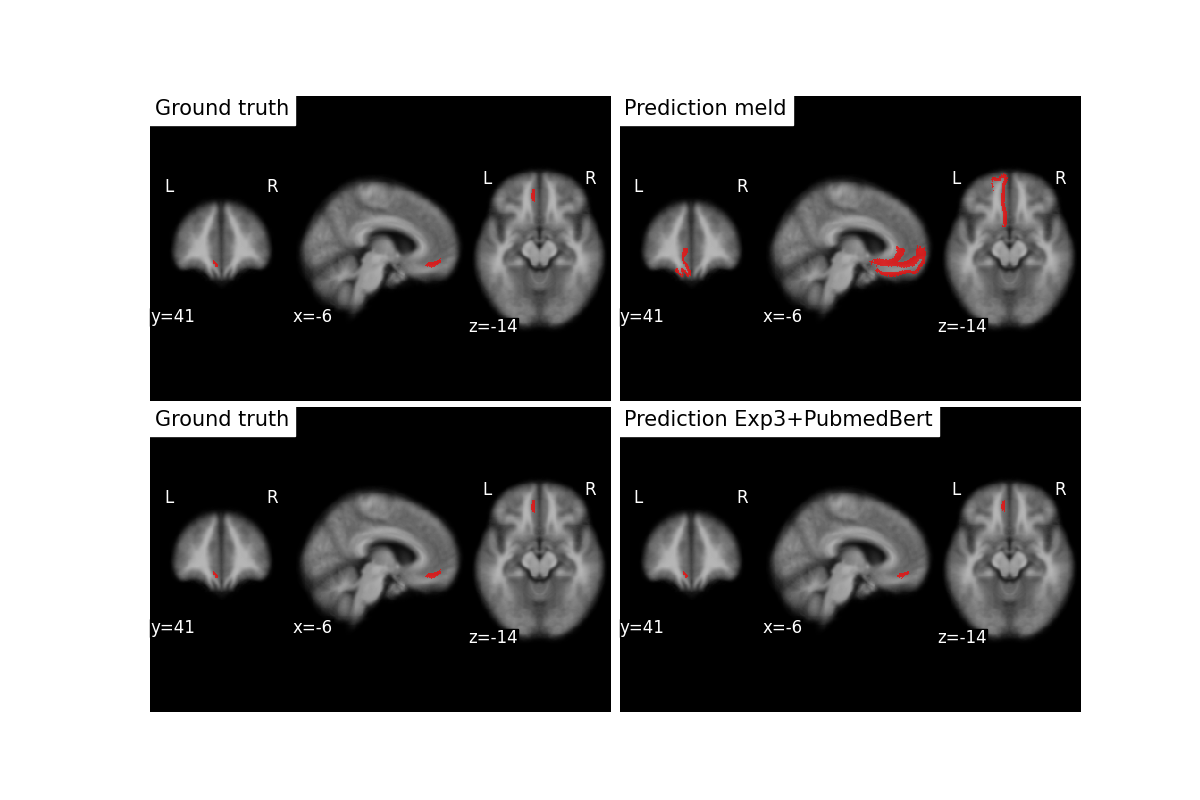
\includegraphics[width=0.9\textwidth]{pictures/MELD_H3_3T_FCD_0002.png}
    \caption{Comparison for subject \texttt{MELD\_H3\_3T\_FCD\_0002}.}
    % \label{fig:qual_example1}
\end{figure}

\begin{figure}[H]
    \centering
    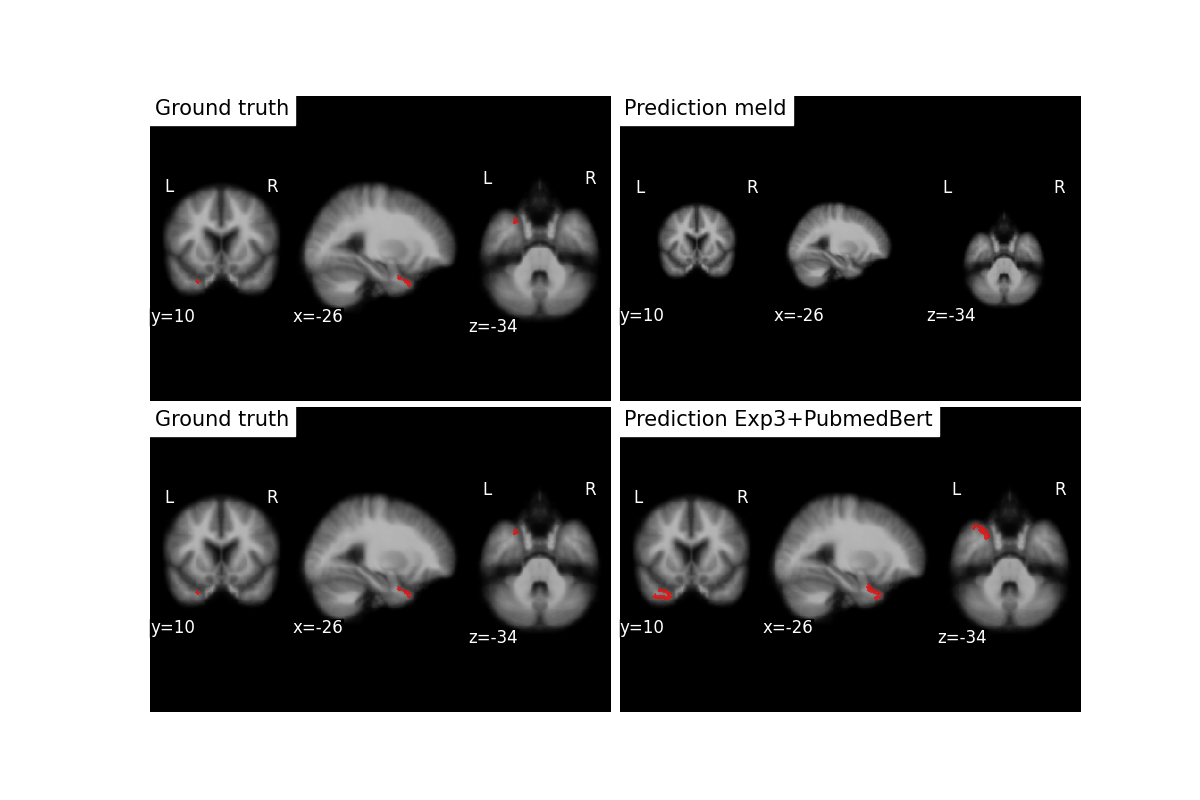
\includegraphics[width=0.9\textwidth]{pictures/MELD_H16_3T_FCD_048.png}
    \caption{Comparison for subject \texttt{MELD\_H16\_3T\_FCD\_048}.}
    % \label{fig:qual_example2}
\end{figure}

Finally, we present an example comparing the same \texttt{Vision+LM} model conditioned on different textual descriptions, namely the \textit{hemi} and \textit{hemi + lobe} prompts.
\begin{figure}[H]
    \centering
    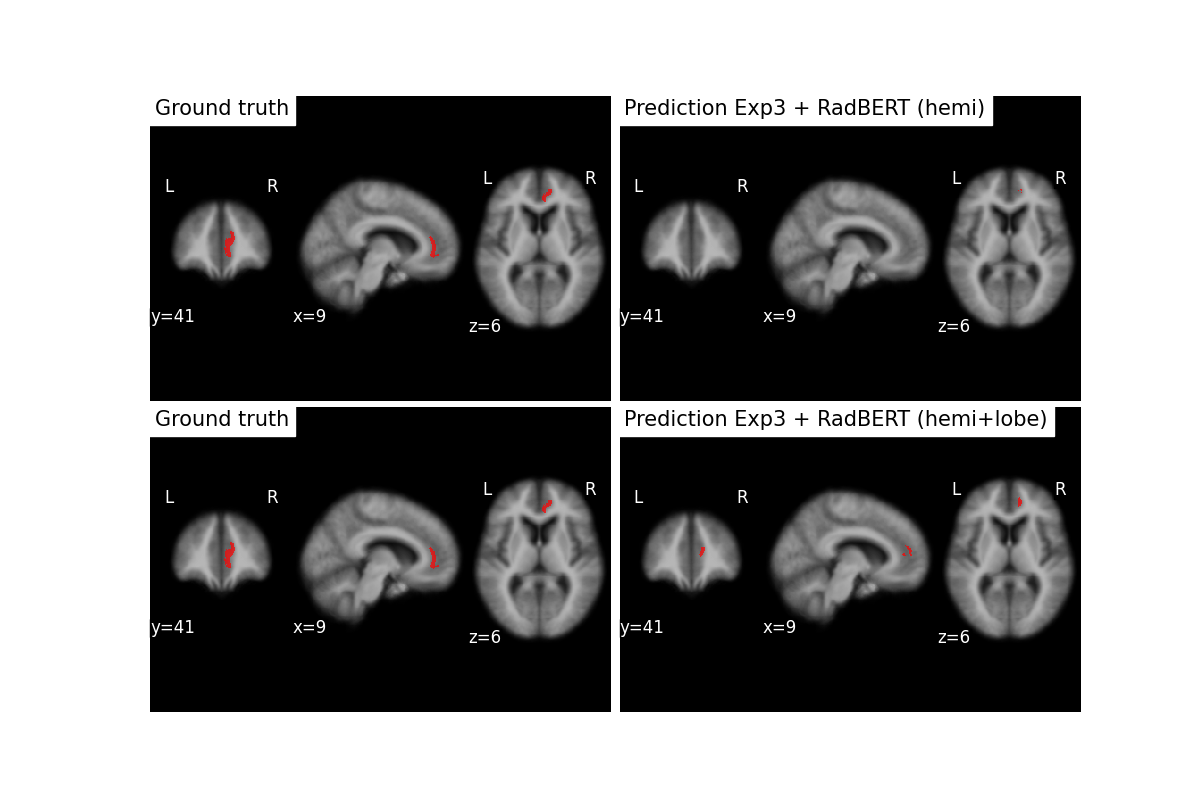
\includegraphics[width=0.9\textwidth]{pictures/MELD_H3_3T_FCD_0018.png}
    \caption{Comparison for subject \texttt{MELD\_H3\_3T\_FCD\_0018}.}
    % \label{fig:qual_example2}
\end{figure}

% \clearpage
\section{Mixed Text}
This chapter investigates training with \textit{mixed text prompts} and the effect of a short decoder warm--up phase.
We start from the \texttt{Vision+LM} architecture and compare two training schedules:
\begin{enumerate}
  \item \textbf{Decoder open from the start}: the \texttt{GuideDecoder} is initialized with pretrained weights from \textit{Vision--only} and optimized from the first epoch.
  \item \textbf{Decoder warm--up (5 epochs)}: the model is initialized from the \texttt{Vision--only} checkpoint; during the first five epochs, we optimize only the text--fusion parameters in the \texttt{GuideDecoder} (self--/cross--attention and the text projection), while the \ac{meld} visual backbone, the text encoder (RadBERT), the SpiralConv--based upsampling path, and the segmentation head remain frozen.
  The choice of five epochs is pragmatic: each experiment uses an ensemble of models, training a single model takes roughly 8 hours, and typical runs span 20--30 epochs; therefore, a 5-epoch warm--up was considered sufficient.
\end{enumerate}

We train the model with different atlas--based prompt variants, where one prompt type is randomly sampled per sample during training.
All experiments in this chapter use \textbf{RadBERT} as the text encoder.
Finally, we evaluate the trained models using intentionally mismatched (incorrect) prompts to assess robustness to prompt variability.


\subsection*{Warm--up vs.\ training from the start}

Based on Tables~\ref{tab:main_cohort_mixed_correct} and \ref{tab:main_cohort_mixed_5_epochs_correct}, introducing a 5-epoch warm--up increases specificity by $\sim$8.8 \ac{p.p.} and sensitivity by about 4.5 \ac{p.p.} on average, while Dice, PPV, and IoU decrease slightly (by about 1--2 \ac{p.p.}).
We interpret this as evidence that the warm--up phase allows the \texttt{GuideDecoder} to first learn how to incorporate the textual prompts and establish stable cross--attention links to the visual embeddings, before updating the full model.

\begin{table}[H]
\centering
\tiny
\caption{Different text types for \textbf{Vision+LM\_mixed} models (values in parentheses indicate 95\% confidence intervals). \emph{Decoder open from the start} — GuideDecoder trained from the first epoch. Main cohort — correct descriptions.}

\label{tab:main_cohort_mixed_correct}
\begin{tabular}{lccccccc}
\textbf{Model} &
\textbf{Text type} &
\textbf{Dice} &
\makecell{\textbf{PPV}\\\textbf{pixels}} &
\makecell{\textbf{(mean)} \\\textbf{PPV} \\\textbf{clusters}} & 
% \makecell{\textbf{(median)} \\\textbf{PPV} \\\textbf{clusters}} & 
\textbf{IoU} & 
\makecell{\textbf{Specificity, \%} \\ (N = 193)}&
\makecell{\textbf{Sensitivity, \%} \\ (N = 259)}\\
\hline
MELD & -- &
\makecell{0.230\\(0.107--0.320)} &
\makecell{0.166\\(0.086--0.220)} &
\colorbox{green!15}{0.515} &
% \makecell{1.000 \\ (1.000-1.000)} &
\makecell{0.130\\(0.057--0.190)} &
\makecell{58.0 (n=112) \\ (51.3--64.8)}&
\makecell{65.6 (n=170) \\ (59.8--71.4)} \\
\hline
Vision--only & -- &
\makecell{0.238\\(0.125--0.313)} &
\makecell{0.198\\(0.130--0.318)} &
0.361 &
\makecell{0.135\\(0.066--0.186)} &
\makecell{31.1 (n=60) \\ (24.9--37.8)} &
\makecell{\colorbox{orange!15}{69.1 (n=179)} \\ (63.3--74.9)} \\
\hline
Vision--only+SA & -- &
\makecell{\colorbox{green!15}{0.256} \\ (0.125--0.326)} &
\makecell{0.204\\ (0.122--0.322)} &
0.333 &
\makecell{\colorbox{green!15}{0.147}\\ (0.067--0.195)} &
\makecell{24.9 (n=48) \\ (19.2--31.1)} &
\makecell{\colorbox{green!15}{70.7 (n=183)} \\ (65.3--76.1)} \\
\hline
Vision+LM\_mixed & 
hemi &  
\makecell{0.235 \\ (0.107--0.294)} &
\makecell{0.222 \\ (0.144--0.303)} &
\colorbox{cyan!15}{0.511} &
% \makecell{1.000 \\ (0.500 -- 1.000)}&
\makecell{0.133 \\ (0.057--0.172)} &
\makecell{79.3 (n=153) \\ (73.6--85.0)} &
\makecell{\colorbox{orange!15}{69.1 (n=179)} \\ (63.3--74.9)} \\
\hline
Vision+LM\_mixed &
lobe\_regions &
\makecell{\colorbox{orange!15}{0.243} \\ (0.081--0.323)} &
\makecell{\colorbox{cyan!15}{0.246} \\ (0.151--0.345)} &
0.491 &
% \makecell{1.000 \\ (0.500 -- 1.000)}&
\makecell{\colorbox{orange!15}{0.138} \\ (0.042--0.193)} &
\makecell{79.3 (n=153) \\ (73.6--85.0)} &
\makecell{66.4 (n=172) \\ (60.6--72.2)} \\
\hline
Vision+LM\_mixed &
\makecell{hemi+ \\ lobe\_regions} &
\makecell{0.241 \\ (0.097--0.312)} &
\makecell{\colorbox{orange!15}{0.235} \\ (0.152--0.346)} &
0.492 &
% \makecell{1.000 \\ (0.500 -- 1.000)}&
\makecell{0.137 \\ (0.051--0.185)} &
\makecell{79.3 (n=153) \\ (73.6--85.0)} &
\makecell{68.7 (n=178) \\ (62.9--74.1)} \\
\hline
Vision+LM\_mixed &
hemi+lobe & 
\makecell{0.241 \\ (0.095--0.321)} &
\makecell{0.233 \\ (0.145--0.335)} &
\colorbox{orange!15}{0.505} &
% \makecell{1.000 \\ (0.500 -- 1.000)}&
\makecell{0.137 \\ (0.050--0.191)} &
\makecell{79.3 (n=153) \\ (73.6--85.0)} &
\makecell{67.2 (n=174) \\ (61.4--73.0)} \\
\hline
Vision+LM\_mixed &
full\_desc &
\makecell{\colorbox{cyan!15}{0.251} \\ (0.124--0.300)} &
\makecell{\colorbox{green!15}{0.256} \\ (0.167--0.351)} &
0.479 &
% \makecell{1.000 \\ (0.667 -- 1.000)}&
\makecell{\colorbox{cyan!15}{0.144} \\ (0.066--0.177)} &
\makecell{79.3 (n=153) \\ (73.6--85.0)} &
\makecell{\colorbox{cyan!15}{69.9 (n=181)} \\ (64.1--75.3)} \\
\hline
\end{tabular}
\vspace{2mm}
\par\noindent\centering
\parbox{0.95\linewidth}{\footnotesize\textit{Note:} For healthy subjects (no lesion present), we use the same textual input for all prompt variants: \textit{``No lesion detected.''}}
\end{table}

\begin{table}[H]
\centering
\tiny
\caption{Different text types for \textbf{Vision+LM\_mixed freeze 5 epochs} models (values in parentheses indicate 95\% confidence intervals). \emph{Decoder warm-up for 5 epochs} — GuideDecoder unfrozen after epoch 5. Main cohort — correct descriptions.}

\label{tab:main_cohort_mixed_5_epochs_correct}
\begin{tabular}{lccccccc}
\textbf{Model} &
\textbf{Text type} &
\textbf{Dice} &
\makecell{\textbf{PPV}\\\textbf{pixels}} &
\makecell{\textbf{(mean)} \\\textbf{PPV} \\\textbf{clusters}} & 
% \makecell{\textbf{(median)} \\\textbf{PPV} \\\textbf{clusters}} & 
\textbf{IoU} & 
\makecell{\textbf{Specificity, \%} \\ (N = 193)}&
\makecell{\textbf{Sensitivity, \%} \\ (N = 259)}\\
\hline
MELD & -- &
\makecell{\colorbox{orange!15}{0.230}\\(0.107--0.320)} &
\makecell{0.166\\(0.086--0.220)} &
\colorbox{green!15}{0.515} &
% \makecell{1.000 \\ (1.000-1.000)} &
\makecell{\colorbox{orange!15}{0.130}\\(0.057--0.190)} &
\makecell{58.0 (n=112) \\ (51.3--64.8)}&
\makecell{65.6 (n=170) \\ (59.8--71.4)} \\
\hline
Vision--only & -- &
\makecell{\colorbox{cyan!15}{0.238}\\(0.125--0.313)} &
\makecell{0.198\\(0.130--0.318)} &
0.361 &
\makecell{\colorbox{cyan!15}{0.135}\\(0.066--0.186)} &
\makecell{31.1 (n=60) \\ (24.9--37.8)} &
\makecell{69.1 (n=179) \\ (63.3--74.9)} \\
\hline
Vision--only+SA & -- &
\makecell{\colorbox{green!15}{0.256} \\ (0.125--0.326)} &
\makecell{0.204\\ (0.122--0.322)} &
0.333 &
\makecell{\colorbox{green!15}{0.147}\\ (0.067--0.195)} &
\makecell{24.9 (n=48) \\ (19.2--31.1)} &
\makecell{70.7 (n=183) \\ (65.3--76.1)} \\
\hline
Vision+LM\_mixed & 
hemi &
\makecell{0.225 \\ (0.131--0.294)} &
\makecell{0.215 \\ (0.137--0.325)} &
0.401 &
% \makecell{0.667 \\ (0.500 -- 1.000)}&
\makecell{0.127 \\ (0.070--0.172)} &
\makecell{88.1 (n=170) \\ (83.4--92.2)} &
\makecell{\colorbox{cyan!15}{73.7 (n=191)} \\ (68.3--79.2)} \\
\hline
Vision+LM\_mixed & 
lobe\_regions &
\makecell{0.207 \\ (0.123--0.330)} &
\makecell{\colorbox{cyan!15}{0.244} \\ (0.160--0.307)} &
\colorbox{orange!15}{0.419} &
% \makecell{0.667 \\ (0.500 -- 1.000)} &
\makecell{0.116 \\ (0.065--0.197)} &
\makecell{88.1 (n=170) \\ (83.4--92.2)} &
\makecell{71.8 (n=186) \\ (66.4--77.2)} \\
\hline
Vision+LM\_mixed & 
\makecell{hemi+ \\lobe\_regions} &
\makecell{0.219 \\ (0.148--0.323)} &
\makecell{\colorbox{orange!15}{0.216} \\ (0.154--0.291)} &
0.392 &
% \makecell{0.667 \\ (0.500 -- 1.000)}&
\makecell{0.123 \\ (0.080--0.192)} &
\makecell{88.1 (n=170) \\ (83.4--92.2)} &
\makecell{\colorbox{orange!15}{73.0 (n=189)} \\ (67.6--78.4)} \\
\hline
Vision+LM\_mixed & 
\makecell{hemi+ \\lobe} &
\makecell{0.228 \\ (0.129--0.321)} &
\makecell{\colorbox{green!15}{0.247} \\ (0.180--0.330)} &
\colorbox{cyan!15}{0.482} &
% \makecell{0.750 \\ (0.500 -- 1.000)}&
\makecell{0.129 \\ (0.069--0.180)} &
\makecell{88.1 (n=170) \\ (83.4--92.2)} &
\makecell{71.0 (n=184) \\ (65.6--76.4)} \\
\hline
Vision+LM\_mixed & 
full\_desc &
\makecell{\colorbox{orange!15}{0.230} \\ (0.140--0.297)} &
\makecell{0.204 \\ (0.141--0.275)} &
0.342 &
% \makecell{0.500 \\ (0.500 -- 1.000)}&
\makecell{\colorbox{orange!15}{0.130} \\ (0.075--0.175)} &
\makecell{88.1 (n=170) \\ (83.4--92.2)} &
\makecell{\colorbox{green!15}{74.5 (n=193)} \\ (69.1--79.9)} \\
\hline
\end{tabular}
\vspace{2mm}
\par\noindent\centering
\parbox{0.95\linewidth}{\footnotesize\textit{Note:} For healthy subjects (no lesion present), we use the same textual input for all prompt variants: \textit{``No lesion detected.''}}
\end{table}

\subsection*{Wrong textual descriptions (Main cohort)}
We now evaluate models with \emph{incorrect} prompts, including the \texttt{no\_text} setting (i.e., the model receives the placeholder string \textit{full\_brain} as input).

Across both Tables~\ref{tab:wrong_main_cohort_mix_no_freeze} and~\ref{tab:wrong_main_cohort_mix_freeze}, models that were trained on correct 
textual descriptions but tested with intentionally incorrect ones still follow a consistent trend. 
Overall, when evaluated with intentionally incorrect prompts, performance decreases as expected, but the degradation is often modest and in some settings remains comparable to that obtained with correct descriptions.
A possible explanation for this behavior is discussed in chapter~\ref{chapter:Discussion}.

Using the \texttt{no\_text} setting (i.e., providing a fixed placeholder prompt, \textit{full brain}, 
for both patients and healthy controls) does not substantially degrade overall performance; 
however, the metrics become consistently worse.
Based on Table~\ref{tab:wrong_main_cohort_mix_no_freeze} and in comparison to evaluation with correct descriptions 
(Table~\ref{tab:main_cohort_mixed_correct}), \textbf{Specificity} decreases by roughly 27 \ac{p.p.}.
A similar pattern is observed for \textbf{Sensitivity}: the \texttt{no\_text} variant detects fewer lesions, 
with sensitivity lower by about 2 \ac{p.p.} compared to using wrong prompts 
(Table~\ref{tab:wrong_main_cohort_mix_freeze}), and by about 4 \ac{p.p.} compared to using correct prompts 
(Table~\ref{tab:main_cohort_mixed_correct}).


Without any linguistic prior, the attention becomes broad and less informative. 
Under strong class imbalance, the model behaves more conservatively and fires only at very high confidence.

\begin{table}[H]
\centering
\tiny
\caption{Different text types with \emph{wrong} descriptions (without freezing). Main cohort — wrong descriptions}
\label{tab:wrong_main_cohort_mix_no_freeze}
\begin{tabular}{lccccccc}
\textbf{Model} &
\textbf{Text type} &
\textbf{Dice} &
\makecell{\textbf{PPV}\\\textbf{pixels}} &
\makecell{\textbf{(mean)} \\\textbf{PPV} \\\textbf{clusters}} & 
% \makecell{\textbf{(median)} \\\textbf{PPV} \\\textbf{clusters}} & 
\textbf{IoU} & 
\makecell{\textbf{Specificity, \%} \\ (N = 193)}&
\makecell{\textbf{Sensitivity, \%} \\ (N = 259)}\\
\hline
MELD & -- &
\makecell{0.230\\(0.107--0.320)} &
\makecell{0.166\\(0.086--0.220)} &
\colorbox{green!15}{0.515} &
% \makecell{1.000 \\ (1.000-1.000)} &
\makecell{0.130\\(0.057--0.190)} &
\makecell{58.0 (n=112) \\ (51.3--64.8)}&
\makecell{65.6 (n=170) \\ (59.8--71.4)} \\
\hline
Vision--only & -- &
\makecell{0.238\\(0.125--0.313)} &
\makecell{0.198\\(0.130--0.318)} &
0.361 &
\makecell{0.135\\(0.066--0.186)} &
\makecell{31.1 (n=60) \\ (24.9--37.8)} &
\makecell{\colorbox{orange!15}{69.1 (n=179)} \\ (63.3--74.9)} \\
\hline
Vision--only+SA & -- &
\makecell{\colorbox{green!15}{0.256} \\ (0.125--0.326)} &
\makecell{0.204\\ (0.122--0.322)} &
0.333 &
\makecell{\colorbox{green!15}{0.147}\\ (0.067--0.195)} &
\makecell{24.9 (n=48) \\ (19.2--31.1)} &
\makecell{\colorbox{green!15}{70.7 (n=183)} \\ (65.3--76.1)} \\
\hline
Vision+LM\_mixed & wrong\_hemi &
\makecell{0.234 \\ (0.109--0.304)} &
\makecell{0.217 \\ (0.144--0.296)} &
\colorbox{cyan!15}{0.509} &
% \makecell{1.000 \\ (0.500 -- 1.000)} &
\makecell{0.133 \\ (0.057--0.179)} &
\makecell{79.3 (n=153) \\ (73.6--85.0)} &
\makecell{\colorbox{cyan!15}{69.5 (n=180)} \\ (63.7--74.9)} \\
\hline
Vision+LM\_mixed & 
\makecell{wrong\_hemi + \\ correct\_lobe\_regions} &
\makecell{0.240 \\ (0.097--0.312)} &
\makecell{\colorbox{green!15}{0.241} \\ (0.152--0.346)} &
0.486 &
% \makecell{1.000 \\ (0.500 -- 1.000)} &
\makecell{0.136 \\ (0.051--0.185)} &
\makecell{79.3 (n=153) \\ (73.6--85.0)} &
\makecell{67.6 (n=175) \\ (61.8--73.4)} \\
\hline
Vision+LM\_mixed & 
\makecell{wrong\_hemi + \\ correct\_lobe} &
\makecell{0.239 \\ (0.088--0.317)} &
\makecell{\colorbox{orange!15}{0.228} \\ (0.146--0.332)} &
\colorbox{orange!15}{0.508} &
% \makecell{1.000 \\ (0.667 -- 1.000)} &
\makecell{0.135 \\ (0.046--0.188)} &
\makecell{79.3 (n=153) \\ (73.6--85.0)} &
\makecell{67.6 (n=175) \\ (61.8--73.4)} \\
\hline
Vision+LM\_mixed & \makecell{wrong\_hemi + \\ wrong\_lobe\_regions} &
\makecell{0.241 \\ (0.098--0.320)} &
\makecell{0.222 \\ (0.147--0.343)} &
0.489 &
% \makecell{1.000 \\ (0.667 -- 1.000)} &
\makecell{0.137 \\ (0.052--0.190)} &
\makecell{79.3 (n=153) \\ (73.6--85.0)} &
\makecell{68.0 (n=176) \\ (62.2--73.7)} \\
\hline
Vision+LM\_mixed & \makecell{wrong\_hemi + \\ wrong\_lobe} &
\makecell{\colorbox{orange!15}{0.243} \\ (0.083--0.317)} &
\makecell{\colorbox{cyan!15}{0.234} \\ (0.148--0.331)} &
0.498 &
% \makecell{1.000 \\ (0.500 -- 1.000)} &
\makecell{\colorbox{orange!15}{0.139} \\ (0.044--0.188)} &
\makecell{79.3 (n=153) \\ (73.6--85.0)} &
\makecell{67.2 (n=174) \\ (61.4--73.0)} \\
\hline
Vision+LM\_mixed & no\_text &
\makecell{\colorbox{cyan!15}{0.249} \\ (0.080--0.296)} &
\makecell{0.192 \\ (0.127--0.289)} &
0.443 &
% \makecell{1.000 \\ (0.500 -- 1.000)} &
\makecell{\colorbox{cyan!15}{0.142} \\ (0.042--0.174)} &
\makecell{52.3 (n=101) \\ (45.1--59.1)} &
\makecell{66.0 (n=171) \\ (60.2--71.8)} \\

\hline
\end{tabular}
\end{table}

A similar effect is observed in Table~\ref{tab:wrong_main_cohort_mix_freeze}.  
Even when models are \emph{trained on correct textual descriptions} but evaluated using deliberately incorrect prompts, 
freezing the decoder for the first 5 epochs again leads to a performance gain. 
This effect is consistently observed across all settings with incorrect textual descriptions, 
except for the \texttt{no\_text} baseline, where \textbf{Specificity} decreases by about 14 \ac{p.p.} 
when compared to the corresponding no-freeze results in Table~\ref{tab:wrong_main_cohort_mix_no_freeze}. 
In contrast, \textbf{Sensitivity} still improves by roughly 2 \ac{p.p.} when decoder freezing is applied.

% This again demonstrates that, when the decoder warm-up is applied, the model becomes less 
% sensitive to misleading or contradictory prompts during evaluation.

\begin{table}[H]
\centering
\tiny
\caption{Different text types with \emph{wrong} descriptions (with 5 frozen epochs). Main cohort — wrong descriptions}
\label{tab:wrong_main_cohort_mix_freeze}
\begin{tabular}{lccccccc}
\textbf{Model} &
\textbf{Text type} &
\textbf{Dice} &
\makecell{\textbf{PPV}\\\textbf{pixels}} &
\makecell{\textbf{(mean)} \\\textbf{PPV} \\\textbf{clusters}} & 
% \makecell{\textbf{(median)} \\\textbf{PPV} \\\textbf{clusters}} & 
\textbf{IoU} & 
\makecell{\textbf{Specificity, \%} \\ (N = 193)}&
\makecell{\textbf{Sensitivity, \%} \\ (N = 259)}\\
\hline
MELD & -- &
\makecell{0.230\\(0.107--0.320)} &
\makecell{0.166\\(0.086--0.220)} &
\colorbox{green!15}{0.515} &
% \makecell{1.000 \\ (1.000-1.000)} &
\makecell{0.130\\(0.057--0.190)} &
\makecell{58.0 (n=112) \\ (51.3--64.8)}&
\makecell{65.6 (n=170) \\ (59.8--71.4)} \\
\hline
Vision--only & -- &
\makecell{\colorbox{orange!15}{0.238}\\(0.125--0.313)} &
\makecell{0.198\\(0.130--0.318)} &
0.361 &
\makecell{\colorbox{cyan!15}{0.135}\\(0.066--0.186)} &
\makecell{31.1 (n=60) \\ (24.9--37.8)} &
\makecell{69.1 (n=179) \\ (63.3--74.9)} \\
\hline
Vision--only+SA & -- &
\makecell{\colorbox{green!15}{0.256} \\ (0.125--0.326)} &
\makecell{0.204\\ (0.122--0.322)} &
0.333 &
\makecell{\colorbox{green!15}{0.147}\\ (0.067--0.195)} &
\makecell{24.9 (n=48) \\ (19.2--31.1)} &
\makecell{70.7 (n=183) \\ (65.3--76.1)} \\
\hline
Vision+LM\_mixed & 
wrong\_hemi &
\makecell{0.231 \\ (0.119--0.287)} &
\makecell{\colorbox{orange!15}{0.207} \\ (0.139--0.303)} &
0.403 &
% \makecell{0.667 \\ (0.500 -- 1.000)} &
\makecell{0.131 \\ (0.063--0.167)} &
\makecell{88.1 (n=170) \\ (83.4--92.2)} &
\makecell{\colorbox{cyan!15}{73.7 (n=191)} \\ (68.3--79.2)} \\
\hline
Vision+LM\_mixed & 
\makecell{wrong\_hemi + \\ correct\_lobe\_regions} &
\makecell{0.216 \\ (0.153--0.322)} &
\makecell{\colorbox{cyan!15}{0.216} \\ (0.153--0.291)} &
0.395 &
% \makecell{0.667 \\ (0.500 -- 1.000)} &
\makecell{0.121 \\ (0.083--0.192)} &
\makecell{88.1 (n=170) \\ (83.4--92.2)} &
\makecell{\colorbox{orange!15}{73.0 (n=189)} \\ (67.6--78.4)} \\
\hline
Vision+LM\_mixed & 
\makecell{wrong\_hemi + \\ correct\_lobe} &
\makecell{0.222 \\ (0.120--0.318)} &
\makecell{\colorbox{green!15}{0.243} \\ (0.166--0.329)} &
\colorbox{cyan!15}{0.479} &
% \makecell{0.800 \\ (0.500 -- 1.000)} &
\makecell{0.125 \\ (0.064--0.189)} &
\makecell{88.1 (n=170) \\ (83.4--92.2)} &
\makecell{70.7 (n=183) \\ (65.3--76.1)} \\
\hline
Vision+LM\_mixed &
\makecell{wrong\_hemi+\\wrong\_lobe\_regions} &
\makecell{0.224 \\ (0.135--0.330)} &
\makecell{\colorbox{orange!15}{0.207} \\ (0.149--0.298)} &
0.378 &
% \makecell{0.667 \\ (0.500 -- 1.000)} &
\makecell{0.126 \\ (0.072--0.198)} &
\makecell{88.1 (n=170) \\ (83.4--92.2)} &
\makecell{\colorbox{green!15}{74.1 (n=192)} \\ (68.7--79.5)} \\
\hline
Vision+LM\_mixed &
\makecell{wrong\_hemi+\\wrong\_lobe} &
\makecell{0.219 \\ (0.114--0.331)} &
\makecell{\colorbox{green!15}{0.243} \\ (0.164--0.346)} &
\colorbox{orange!15}{0.470} &
% \makecell{0.667 \\ (0.500 -- 1.000)} &
\makecell{0.123 \\ (0.060--0.198)} &
\makecell{88.1 (n=170) \\ (83.4--92.2)} &
\makecell{71.0 (n=184) \\ (65.6--76.4)} \\
\hline
Vision+LM\_mixed & 
no\_text &
\makecell{\colorbox{cyan!15}{0.245} \\ (0.102--0.295)} &
\makecell{0.205 \\ (0.132--0.292)} &
0.384 &
% \makecell{1.000 \\ (0.500 -- 1.000)} &
\makecell{\colorbox{cyan!15}{0.140} \\ (0.054--0.173)} &
\makecell{38.3 (n=74) \\ (31.6--45.1)} &
\makecell{68.3 (n=177) \\ (62.5--74.1)} \\
\hline
\end{tabular}
\end{table}

Thus, the warm-up phase provides a consistent benefit: it prevents the decoder from immediately 
overfitting to noisy textual cues and encourages the model to extract whatever useful 
structural information is present, even when the text itself is incorrect.

% However not all incorrect prompts are equally harmful. Prompts that are \emph{contradictory} to the image (\texttt{wrong\_hemi}) degrade performance the most. Inexact but \emph{partially informative} prompts (e.g., rough lobe hints) can still help by providing a weak localization prior. Compared with \texttt{no\_text}, even a rough prompt supplies enough context to stabilize attention and yields better overall metrics.


\subsection*{Wrong textual descriptions (Independent cohort)}
On the independent cohort (Tables~\ref{tab:independent_cohort_mixed}--\ref{tab:wrong_independent_cohort_mix_freeze}), 
for both correct and incorrect prompts, the model with a 5-epoch decoder freeze generally detects 
$\sim$5 \ac{p.p.} more lesions (higher \textbf{Sensitivity}).  
For most text--description settings, this increase in detected lesions does not substantially 
degrade segmentation quality: several segmentation metrics (\textbf{Dice}, \textbf{IoU}, and \textbf{PPV}) remain stable or even improve 
slightly compared to the non-frozen model. 
For the \texttt{hemi + lobe\_regions} and \texttt{full\_desc} prompts, we observe a noticeable decrease 
in segmentation quality (5--11 \ac{p.p.} in Dice and 5--7 \ac{p.p.} in IoU).  
However, these decreases are offset by a consistent improvement in lesion detection, which remains 
the primary objective in this setting.

\begin{table}[H]
    \centering
    \tiny
    \caption{Different text types for \textbf{Vision+LM\_mixed} models (values in parentheses indicate 95\% confidence intervals). \emph{Decoder open from the start} — GuideDecoder trained from the first epoch. Independent cohort — correct descriptions.}
    
    \label{tab:independent_cohort_mixed}
    \begin{tabular}{lccccccc}
    \textbf{Model} &
    \textbf{Text type} &
    \textbf{Dice} &
    \makecell{\textbf{PPV}\\\textbf{pixels}} &
    \makecell{\textbf{(mean)} \\\textbf{PPV} \\\textbf{clusters}} & 
    % \makecell{\textbf{(median)} \\\textbf{PPV} \\\textbf{clusters}} & 
    \textbf{IoU} & 
    \makecell{\textbf{Specificity, \%} \\ (N = 83)}&
    \makecell{\textbf{Sensitivity, \%} \\ (N = 82)}\\
    \hline
    MELD & -- &
    \makecell{0.358\\(0.209--0.465)} &
    \makecell{0.261\\(0.142--0.428)} &
    0.464 &
    % \makecell{1.000\\(1.000--1.000)} &
    \makecell{0.218\\(0.117--0.303)} &
    \makecell{55.4 (n=46) \\ (44.6--66.3)} & 
    \makecell{\colorbox{orange!15}{69.5 (n=57)} \\ (59.8--79.3)} \\
    \hline
    Vision--only & -- &
    \makecell{0.376\\(0.238--0.529)} &
    \makecell{\colorbox{orange!15}{0.443}\\(0.243--0.619)} &
    0.350 &
    \makecell{0.232\\(0.138--0.359)} &
    \makecell{39.8 (n=33) \\ (28.9--50.6)} &
    \makecell{\colorbox{green!15}{73.2 (n=60)} \\ (63.4--82.9)} \\
    \hline
    Vision--only+SA & -- &
    \makecell{0.342\\ (0.155--0.494)} &
    \makecell{0.381\\ (0.177--0.651)} &
    0.379 &
    \makecell{0.206\\ (0.084--0.328)} &
    \makecell{37.3 (n=31) \\ (27.7--48.2)} &
    \makecell{\colorbox{orange!15}{69.5 (n=57)} \\ (59.8--79.3)} \\
    \hline
    Vision+LM\_mixed & 
    hemi &  
    \makecell{\colorbox{green!15}{0.430} \\ (0.067--0.515)} &
    \makecell{0.429 \\ (0.181--0.610)} &
    0.604 &
    % \makecell{1.000 \\ (1.000 -- 1.000)} &
    \makecell{\colorbox{green!15}{0.274} \\ (0.035--0.347)} &
    \makecell{89.2 (n=74) \\ (81.9--95.2)} & 
    \makecell{68.3 (n=56) \\ (57.3--78.0)} \\
    \hline
    Vision+LM\_mixed &
    lobe\_regions &
    \makecell{0.374 \\ (0.177--0.496)} &
    \makecell{\colorbox{cyan!15}{0.486} \\ (0.224--0.670)} &
    \colorbox{green!15}{0.656} &
    % \makecell{1.000 \\ (1.000 -- 1.000)} &
    \makecell{0.230 \\ (0.097--0.330)} &
    \makecell{89.2 (n=74) \\ (81.9--95.2)} & 
    \makecell{68.3 (n=56) \\ (57.3--78.0)} \\
    \hline
    Vision+LM\_mixed & 
    \makecell{hemi+ \\lobe\_regions} &
    \makecell{\colorbox{orange!15}{0.400} \\ (0.222--0.501)} &
    \makecell{\colorbox{green!15}{0.515} \\ (0.242--0.668)} &
    \colorbox{orange!15}{0.616} &
    % \makecell{1.000 \\ (0.500 -- 1.000)} &
    \makecell{\colorbox{orange!15}{0.250} \\ (0.125--0.334)} &
    \makecell{89.2 (n=74) \\ (81.9--95.2)} & 
    \makecell{\colorbox{orange!15}{69.5 (n=57)} \\ (59.8--79.3)} \\
    \hline
    Vision+LM\_mixed &
    hemi+lobe & 
    \makecell{0.380 \\ (0.119--0.498)} &
    \makecell{\colorbox{green!15}{0.515} \\ (0.073--0.655)} &
    0.613 &
    % \makecell{1.000 \\ (1.000 -- 1.000)} &
    \makecell{0.234 \\ (0.064--0.331)} &
    \makecell{89.2 (n=74) \\ (81.9--95.2)} & 
    \makecell{65.9 (n=54) \\ (54.9--75.6)} \\
    \hline
    Vision+LM\_mixed &
    full\_desc &
    \makecell{\colorbox{cyan!15}{0.402} \\ (0.271--0.486)} &
    \makecell{\colorbox{green!15}{0.515} \\ (0.311--0.682)} &
    \colorbox{cyan!15}{0.626} &
    % \makecell{1.000 \\ (1.000 -- 1.000)} &
    \makecell{\colorbox{cyan!15}{0.251} \\ (0.156--0.321)} &
    \makecell{89.2 (n=74) \\ (81.9--95.2)} & 
    \makecell{\colorbox{cyan!15}{70.7 (n=58)} \\ (61.0--80.5)} \\
    \hline
    \end{tabular}
    \end{table}
    
    \begin{table}[ht]
    \centering
    \tiny
    \caption{Different text types for \textbf{Vision+LM\_mixed freeze 5 epochs} models (values in parentheses indicate 95\% confidence intervals). \emph{Decoder warm-up for 5 epochs} — GuideDecoder unfrozen after epoch 5. Independent cohort — correct descriptions.}
    
    \label{tab:main_cohort_mixed}
    \begin{tabular}{lccccccc}
    \textbf{Model} &
    \textbf{Text type} &
    \textbf{Dice} &
    \makecell{\textbf{PPV}\\\textbf{pixels}} &
    \makecell{\textbf{(mean)} \\\textbf{PPV} \\\textbf{clusters}} & 
    % \makecell{\textbf{(median)} \\\textbf{PPV} \\\textbf{clusters}} & 
    \textbf{IoU} & 
    \makecell{\textbf{Specificity, \%} \\ (N = 83)}&
    \makecell{\textbf{Sensitivity, \%} \\ (N = 82)}\\
    \hline
    MELD & -- &
    \makecell{0.358\\(0.209--0.465)} &
    \makecell{0.261\\(0.142--0.428)} &
    0.464 &
    % \makecell{1.000\\(1.000--1.000)} &
    \makecell{0.218\\(0.117--0.303)} &
    \makecell{55.4 (n=46) \\ (44.6--66.3)} & 
    \makecell{69.5 (n=57) \\ (59.8--79.3)} \\
    \hline
    Vision--only & -- &
    \makecell{\colorbox{cyan!15}{0.376}\\(0.238--0.529)} &
    \makecell{\colorbox{cyan!15}{0.443}\\(0.243--0.619)} &
    0.350 &
    \makecell{\colorbox{cyan!15}{0.232}\\(0.138--0.359)} &
    \makecell{39.8 (n=33) \\ (28.9--50.6)} &
    \makecell{73.2 (n=60) \\ (63.4--82.9)} \\
    \hline
    Vision--only+SA & -- &
    \makecell{0.342\\ (0.155--0.494)} &
    \makecell{0.381\\ (0.177--0.651)} &
    0.379 &
    \makecell{0.206\\ (0.084--0.328)} &
    \makecell{37.3 (n=31) \\ (27.7--48.2)} &
    \makecell{69.5 (n=57) \\ (59.8--79.3)} \\
    \hline
    Vision+LM\_mixed & 
    hemi &
    \makecell{\colorbox{orange!15}{0.368} \\ (0.248--0.505)} &
    \makecell{\colorbox{orange!15}{0.406} \\ (0.218--0.596)} &
    \colorbox{cyan!15}{0.489} &
    % \makecell{1.000 \\ (0.500 -- 1.000)}&
    \makecell{\colorbox{orange!15}{0.225} \\ (0.141--0.338)} &
    \makecell{94.0 (n=78) \\ (88.0--98.8)} &
    \makecell{\colorbox{orange!15}{74.4 (n=61)} \\ (64.6--84.1)} \\
    \hline
    Vision+LM\_mixed & 
    lobe\_regions &
    \makecell{0.335 \\ (0.144--0.474)} &
    \makecell{0.338 \\ (0.168--0.543)} &
    \colorbox{orange!15}{0.486} &
    % \makecell{1.000 \\ (0.500 -- 1.000)}&
    \makecell{0.201 \\ (0.077--0.311)} &
    \makecell{94.0 (n=78) \\ (88.0--98.8)} &
    \makecell{72.0 (n=59) \\ (62.2--81.7)} \\
    \hline
    Vision+LM\_mixed & 
    \makecell{hemi+ \\lobe\_regions} &
    \makecell{0.332 \\ (0.183--0.477)} &
    \makecell{0.343 \\ (0.174--0.576)} &
    0.474 &
    % \makecell{1.000 \\ (0.500 -- 1.000)}&
    \makecell{0.199 \\ (0.101--0.313)} &
    \makecell{94.0 (n=78) \\ (88.0--98.8)} &
    \makecell{\colorbox{cyan!15}{75.6 (n=62)} \\ (65.9--84.1)} \\
    \hline
    Vision+LM\_mixed & 
    hemi+lobe &
    \makecell{\colorbox{green!15}{0.400} \\ (0.162--0.507)} &
    \makecell{\colorbox{green!15}{0.462} \\ (0.239--0.672)} &
    \colorbox{green!15}{0.586} &
    % \makecell{1.000 \\ (0.750 -- 1.000)}&
    \makecell{\colorbox{green!15}{0.250} \\ (0.088--0.340)} &
    \makecell{94.0 (n=78) \\ (88.0--98.8)} &
    \makecell{\colorbox{orange!15}{74.4 (n=61)} \\ (64.6--84.1)} \\
    \hline
    Vision+LM\_mixed & 
    full\_desc &
    \makecell{0.305 \\ (0.210--0.478)} &
    \makecell{0.326 \\ (0.164--0.651)} &
    0.306 &
    % \makecell{1.000 \\ (0.500 -- 1.000)}&
    \makecell{0.180 \\ (0.117--0.314)} &
    \makecell{94.0 (n=78) \\ (88.0--98.8)} &
    \makecell{\colorbox{green!15}{78.0 (n=64)} \\ (68.3--86.6)} \\
    
    \hline
    \end{tabular}
    \end{table}

\begin{table}[H]
    \centering
    \tiny
    \caption{Different text types with \emph{wrong} descriptions (without freezing). Independent cohort — wrong descriptions}
    \label{tab:wrong_independent_cohort_mix_no_freeze}
    \begin{tabular}{lccccccc}
    \textbf{Model} &
    \textbf{Text type} &
    \textbf{Dice} &
    \makecell{\textbf{PPV}\\\textbf{pixels}} &
    \makecell{\textbf{(mean)}\\\textbf{PPV}\\\textbf{clusters}} &
    % \makecell{\textbf{(median)}\\\textbf{PPV}\\\textbf{clusters}} &
    \textbf{IoU} &
    \makecell{\textbf{Specificity, \%} \\ (N = 83)}&
    \makecell{\textbf{Sensitivity, \%} \\ (N = 82)}\\
    \hline
    MELD & -- &
    \makecell{0.358\\(0.209--0.465)} &
    \makecell{0.261\\(0.142--0.428)} &
    0.464 &
    % \makecell{1.000\\(1.000--1.000)} &
    \makecell{0.218\\(0.117--0.303)} &
    \makecell{55.4 (n=46) \\ (44.6--66.3)} & 
    \makecell{\colorbox{cyan!15}{69.5 (n=57)} \\ (59.8--79.3)} \\
    \hline
    Vision--only & -- &
    \makecell{0.376\\(0.238--0.529)} &
    \makecell{0.443\\(0.243--0.619)} &
    0.350 &
    \makecell{0.232\\(0.138--0.359)} &
    \makecell{39.8 (n=33) \\ (28.9--50.6)} &
    \makecell{\colorbox{green!15}{73.2 (n=60)} \\ (63.4--82.9)} \\
    \hline
    Vision--only+SA & -- &
    \makecell{0.342\\ (0.155--0.494)} &
    \makecell{0.381\\ (0.177--0.651)} &
    0.379 &
    \makecell{0.206\\ (0.084--0.328)} &
    \makecell{37.3 (n=31) \\ (27.7--48.2)} &
    \makecell{\colorbox{cyan!15}{69.5 (n=57)} \\ (59.8--79.3)} \\
    \hline
    Vision+LM\_mixed &
    wrong\_hemi &
    \makecell{\colorbox{cyan!15}{0.421} \\ (0.067--0.520)} &
    \makecell{0.432 \\ (0.179--0.609)} &
    0.604 &
    % \makecell{1.000 \\ (1.000 -- 1.000)} &
    \makecell{\colorbox{cyan!15}{0.267} \\ (0.035--0.352)} &
    \makecell{89.2 (n=74) \\ (81.9--95.2)} &
    \makecell{\colorbox{orange!15}{68.3 (n=56)} \\ (57.3--78.0)} \\
    \hline
    Vision+LM\_mixed &
    \makecell{wrong\_hemi + \\ correct\_lobe\_regions} &
    \makecell{0.392 \\ (0.214--0.503)} &
    \makecell{\colorbox{green!15}{0.515} \\ (0.240--0.675)} &
    \colorbox{cyan!15}{0.625} &
    % \makecell{1.000 \\ (1.000 -- 1.000)} &
    \makecell{0.244 \\ (0.120--0.336)} &
    \makecell{89.2 (n=74) \\ (81.9--95.2)} &
    \makecell{\colorbox{cyan!15}{69.5 (n=57)} \\ (59.8--79.3)} \\
    \hline
    Vision+LM\_mixed &
    \makecell{wrong\_hemi + \\ correct\_lobe} &
    \makecell{0.378 \\ (0.119--0.492)} &
    \makecell{\colorbox{cyan!15}{0.509} \\ (0.073--0.658)} &
    0.613 &
    % \makecell{1.000 \\ (1.000 -- 1.000)} &
    \makecell{0.233 \\ (0.063--0.326)} &
    \makecell{89.2 (n=74) \\ (81.9--95.2)} &
    \makecell{65.9 (n=54) \\ (54.9--75.6)} \\
    \hline
    Vision+LM\_mixed &
    \makecell{wrong\_hemi + \\ wrong\_lobe\_regions} &
    \makecell{\colorbox{green!15}{0.433} \\ (0.258--0.515)} &
    \makecell{0.475 \\ (0.256--0.676)} &
    \colorbox{green!15}{0.660} &
    % \makecell{1.000 \\ (1.000 -- 1.000)} &
    \makecell{\colorbox{green!15}{0.276} \\ (0.148--0.346)} &
    \makecell{89.2 (n=74) \\ (81.9--95.2)} &
    \makecell{\colorbox{cyan!15}{69.5 (n=57)} \\ (59.8--79.3)} \\
    \hline
    Vision+LM\_mixed &
    \makecell{wrong\_hemi + \\ wrong\_lobe} &
    \makecell{0.388 \\ (0.147--0.501)} &
    \makecell{0.481 \\ (0.154--0.672)} &
    \colorbox{orange!15}{0.617} &
    % \makecell{1.000 \\ (1.000 -- 1.000)} &
    \makecell{0.241 \\ (0.079--0.334)} &
    \makecell{89.2 (n=74) \\ (81.9--95.2)} &
    \makecell{67.1 (n=55) \\ (56.1--76.8)} \\
    \hline
    Vision+LM\_mixed &
    no\_text &
    \makecell{\colorbox{orange!15}{0.397} \\ (0.138--0.502)} &
    \makecell{\colorbox{orange!15}{0.507} \\ (0.151--0.647)} &
    0.549 &
    % \makecell{1.000 \\ (1.000 -- 1.000)} &
    \makecell{\colorbox{orange!15}{0.248} \\ (0.074--0.335)} &
    \makecell{68.7 (n=57) \\ (59.0--78.3)} & 
    \makecell{65.9 (n=54) \\ (54.9--75.6)} \\
    \hline
    \end{tabular}
\end{table}
    
We also compare two key text--description types, \texttt{hemi+lobe} and \texttt{hemi+lobe\_regions},
under both training strategies (with and without decoder warm-up). For models trained \emph{without} decoder warm-up, the \texttt{hemi+lobe\_regions} setting consistently produces higher segmentation quality:
Dice and IoU improve by $\sim$2-3 \ac{p.p.}, and Sensitivity increases by $\sim$2-4 \ac{p.p.} compared to
\texttt{hemi+lobe}. The same trend is seen in the evaluation of the incorrect text condition, where we compare
\texttt{wrong\_hemi + wrong\_lobe} with \texttt{wrong\_hemi + wrong\_lobe\_regions}. However, for models trained \emph{with} 5-epoch warm-up, the situation is the opposite. 
In this case, the \texttt{hemi+lobe} model provides higher segmentation accuracy, outperforming \texttt{hemi+lobe\_regions} 
by $\sim$3-7 \ac{p.p.} in Dice and IoU, although with a slight decrease in Sensitivity (typically 1-2 \ac{p.p.}).

\begin{table}[H]
    \centering
    \tiny
    \caption{Different text types with \emph{wrong} descriptions (with 5 frozen epochs). Independent cohort — wrong descriptions}
    \label{tab:wrong_independent_cohort_mix_freeze}
    \begin{tabular}{lccccccc}
    \textbf{Model} &
    \textbf{Text type} &
    \textbf{Dice} &
    \makecell{\textbf{PPV}\\\textbf{pixels}} &
    \makecell{\textbf{(mean)}\\\textbf{PPV}\\\textbf{clusters}} &
    % \makecell{\textbf{(median)}\\\textbf{PPV}\\\textbf{clusters}} &
    \textbf{IoU} &
    \makecell{\textbf{Specificity, \%} \\ (N = 83)}&
    \makecell{\textbf{Sensitivity, \%} \\ (N = 82)}\\
    \hline
    MELD & -- &
    \makecell{0.358\\(0.209--0.465)} &
    \makecell{0.261\\(0.142--0.428)} &
    0.464 &
    % \makecell{1.000\\(1.000--1.000)} &
    \makecell{0.218\\(0.117--0.303)} &
    \makecell{55.4 (n=46) \\ (44.6--66.3)} & 
    \makecell{69.5 (n=57) \\ (59.8--79.3)} \\
    \hline
    Vision--only & -- &
    \makecell{\colorbox{cyan!15}{0.376}\\(0.238--0.529)} &
    \makecell{\colorbox{cyan!15}{0.443}\\(0.243--0.619)} &
    0.350 &
    \makecell{\colorbox{cyan!15}{0.232}\\(0.138--0.359)} &
    \makecell{39.8 (n=33) \\ (28.9--50.6)} &
    \makecell{\colorbox{cyan!15}{73.2 (n=60)} \\ (63.4--82.9)} \\
    \hline
    Vision--only+SA & -- &
    \makecell{0.342\\ (0.155--0.494)} &
    \makecell{0.381\\ (0.177--0.651)} &
    0.379 &
    \makecell{0.206\\ (0.084--0.328)} &
    \makecell{37.3 (n=31) \\ (27.7--48.2)} &
    \makecell{69.5 (n=57) \\ (59.8--79.3)} \\
    \hline
    Vision+LM\_mixed &
    wrong\_hemi &
    \makecell{\colorbox{orange!15}{0.368} \\ (0.273--0.499)} &
    \makecell{\colorbox{orange!15}{0.382} \\ (0.220--0.558)} &
    \colorbox{orange!15}{0.471} &
    % \makecell{1.000 \\ (0.500 -- 1.000)} &
    \makecell{\colorbox{orange!15}{0.225} \\ (0.158--0.333)} &
    \makecell{94.0 (n=78) \\ (88.0--98.8)} &
    \makecell{\colorbox{green!15}{74.4 (n=61)} \\ (64.6--84.1)} \\
    \hline
    Vision+LM\_mixed &
    \makecell{wrong\_hemi + \\ correct\_lobe\_regions} &
    \makecell{0.321 \\ (0.163--0.456)} &
    \makecell{0.336 \\ (0.152--0.545)} &
    \colorbox{orange!15}{0.471} &
    % \makecell{1.000 \\ (0.500 -- 1.000)} &
    \makecell{0.192 \\ (0.089--0.296)} &
    \makecell{94.0 (n=78) \\ (88.0--98.8)} &
    \makecell{\colorbox{green!15}{74.4 (n=61)} \\ (64.6--84.1)} \\
    \hline
    Vision+LM\_mixed &
    \makecell{wrong\_hemi + \\ correct\_lobe} &
    \makecell{\colorbox{green!15}{0.401} \\ (0.129--0.507)} &
    \makecell{\colorbox{green!15}{0.448} \\ (0.240--0.676)} &
    \colorbox{green!15}{0.578} &
    % \makecell{1.000 \\ (0.500 -- 1.000)} &
    \makecell{\colorbox{green!15}{0.253} \\ (0.069--0.340)} &
    \makecell{94.0 (n=78) \\ (88.0--98.8)} &
    \makecell{\colorbox{green!15}{74.4 (n=61)} \\ (64.6--84.1)} \\
    \hline
    Vision+LM\_mixed &
    \makecell{wrong\_hemi + \\ wrong\_lobe\_regions} &
    \makecell{0.325 \\ (0.196--0.458)} &
    \makecell{0.338 \\ (0.205--0.619)} &
    0.444 &
    % \makecell{1.000 \\ (0.500 -- 1.000)} &
    \makecell{0.194 \\ (0.109--0.297)} &
    \makecell{94.0 (n=78) \\ (88.0--98.8)} &
    \makecell{\colorbox{green!15}{74.4 (n=61)} \\ (64.6--84.1)} \\
    \hline
    Vision+LM\_mixed &
    \makecell{wrong\_hemi + \\ wrong\_lobe} &
    \makecell{0.353 \\ (0.137--0.489)} &
    \makecell{0.374 \\ (0.245--0.622)} &
    \colorbox{cyan!15}{0.551} &
    % \makecell{1.000 \\ (0.500 -- 1.000)} &
    \makecell{0.214 \\ (0.074--0.324)} &
    \makecell{94.0 (n=78) \\ (88.0--98.8)} &
    \makecell{\colorbox{orange!15}{72.0 (n=59)} \\ (62.2--81.7)} \\
    \hline
    Vision+LM\_mixed &
    no\_text &
    \makecell{0.345 \\ (0.108--0.453)} &
    \makecell{0.349 \\ (0.156--0.567)} &
    0.406 &
    % \makecell{1.000 \\ (0.500 -- 1.000)} &
    \makecell{0.209 \\ (0.058--0.292)} &
    \makecell{47.0 (n=39) \\ (36.1--57.8)} &
    \makecell{64.6 (n=53) \\ (53.7--74.4)} \\
    \hline
    \end{tabular}
\end{table}

These results suggest that the warm-up strategy is preferable for practical use.
In real clinical workflows, coarse anatomical labels are far more common than
precise region-level descriptions, and in such scenarios the warm-up model provides
more reliable segmentation accuracy, even if this comes with a slight reduction in
the number of detected lesions.

% \clearpage
% \subsection*{Mixed Text Part 2}
% In this chapter, we conducted two additional experiments using the Mixed model with several different text description types. Notably, for the “no text” condition we did not provide a fixed phrase such as “No lesion detected.” Instead, we randomly generated a text description composed of a hemisphere name and a lobe name. Each part was sampled according to predefined probabilities, computed from the training-set distribution, as shown below:

% \begin{verbatim}
% {
% "hemisphere_text": {
% "Right Hemisphere": 0.5047923322683706,
% "Left Hemisphere": 0.4952076677316294
% },
% "lobe_text": {
% "Frontal lobe": 0.41533546325878595,
% "Subcortical nuclei": 0.10862619808306709,
% "Limbic lobe": 0.35782747603833864,
% "Temporal lobe": 0.19488817891373802,
% "Occipital lobe": 0.20447284345047922,
% "Parietal lobe": 0.268370607028754,
% "Subcallosal Cortex": 0.04792332268370607,
% "Insular lobe": 0.07028753993610223,
% "Lateral Ventricle": 0.022364217252396165,
% "Brain-Stem": 0.012779552715654952,
% "Central Opercular Cortex": 0.04472843450479233
% }
% }
% \end{verbatim}

% We additionally introduced a new text description type, dominant lobe. For each patient, we converted the detailed lobe-region annotations into a higher-level lobe category. The atlas we used provided percentage overlaps between the lesion and individual regions; these percentages were summed across regions belonging to the same anatomical lobe. The lobe with the highest cumulative percentage was selected as the dominant lobe for that patient. The final text contained only the lobe name without the percentage values.

% The second experiment used the same Mixed model architecture but removed all spatial augmentations and excluded healthy control patients from both training and testing in order to assess how these factors influence overall performance. For the language component, we used the PubMedBERT pretrained model.

% Tables \ref{tab:meld_models_pumbed_main} and \ref{tab:bonn_models_pumbed_main} summarize the results. Dice and IoU metrics differ by no more than 1–2\% across text types, and Sensitivity shows a similar trend. For PPV\textsubscript{pixels} and PPV\textsubscript{clusters}, the values in Table \ref{tab:bonn_models_pumbed_main} are consistently higher, suggesting that training exclusively on FCD patients helps the model better identify true-positive pixels and reduce the number of false positives.

% \begin{table}[H]
% \tiny
% \begin{threeparttable}
% \centering
% \caption{Performance of Exp3\_mixed under different text conditions (MELD dataset).}
% \label{tab:meld_models_pumbed_main}
% \begin{tabular}{lcccccccc}
% \textbf{Model} &
% \textbf{Text type} &
% \textbf{Dice} &
% \textbf{\makecell{PPV \\ pixels}} &
% \textbf{\makecell{PPV \\ clusters \\ (mean)}} &
% \textbf{\makecell{PPV \\ clusters \\ (median)}} &
% \textbf{IoU} &
% \textbf{\makecell{Sensitivity, \% \\ (N = 259)}} &
% \textbf{\makecell{Specificity, \% \\ (N = 193)}} \\
% \midrule

% Exp3\_mixed & hemisphere &
% \makecell{\colorbox{cyan!15}{0.248}\\(0.154--0.318)} &
% \makecell{0.194\\(0.141--0.300)} &
% \colorbox{orange!15}{0.260} &
% \makecell{1.000\\(0.500--1.000)} &
% \makecell{\colorbox{cyan!15}{0.141}\\(0.083--0.189)} &
% \makecell{\colorbox{cyan!15}{72.2 (n=187)} \\ (66.8--77.6)} &
% \makecell{8.3 (n=16) \\ (4.7--12.4)} \\
% \hline
% Exp3\_mixed & lobe &
% \makecell{\colorbox{orange!15}{0.245}\\(0.170--0.324)} &
% \makecell{\colorbox{green!15}{0.209}\\(0.139--0.320)} &
% \colorbox{cyan!15}{0.274} &
% \makecell{1.000\\(0.500--1.000)} &
% \makecell{\colorbox{orange!15}{0.139}\\(0.093--0.193)} &
% \makecell{\colorbox{green!15}{72.6 (n=188)} \\ (67.2--78.0)} &
% \makecell{8.3 (n=16) \\ (4.7--12.4)} \\
% \hline
% Exp3\_mixed & dominant\_lobe &
% \makecell{\colorbox{orange!15}{0.245}\\(0.158--0.324)} &
% \makecell{\colorbox{green!15}{0.209}\\(0.133--0.298)} &
% 0.258 &
% \makecell{1.000\\(0.600--1.000)} &
% \makecell{\colorbox{orange!15}{0.139}\\(0.086--0.193)} &
% \makecell{\colorbox{cyan!15}{72.2 (n=187)} \\ (66.8--77.6)} &
% \makecell{8.3 (n=16) \\ (4.7--12.4)} \\
% \hline
% Exp3\_mixed & hemisphere\_lobe &
% \makecell{0.223\\(0.100--0.304)} &
% \makecell{\colorbox{cyan!15}{0.206}\\(0.129--0.306)} &
% \colorbox{green!15}{0.311} &
% \makecell{1.000\\(0.667--1.000)} &
% \makecell{0.126\\(0.053--0.179)} &
% \makecell{68.0 (n=176) \\ (62.2--73.7)} &
% \makecell{8.3 (n=16) \\ (4.7--12.4)} \\
% \hline
% Exp3\_mixed & no text &
% \makecell{\colorbox{green!15}{0.250}\\(0.146--0.323)} &
% \makecell{\colorbox{orange!15}{0.204}\\(0.140--0.299)} &
% 0.190 &
% \makecell{1.000\\(0.500--1.000)} &
% \makecell{\colorbox{green!15}{0.143}\\(0.079--0.192)} &
% \makecell{\colorbox{orange!15}{71.4 (n=185)} \\ (66.0--76.8)} &
% \makecell{1.0 (n=2) \\ (0.0--2.6)}\\
% \bottomrule
% \end{tabular}
% \end{threeparttable}
% \end{table}

% A notable observation concerns Specificity in Table \ref{tab:meld_models_pumbed_main}, which is extremely low. This occurs because a pretrained decoder was not used, and healthy control patients were provided with incorrect, randomly generated text descriptions. Consequently, the model performs poorly on identifying healthy cases in all settings. Moreover, differences between text types are small, indicating that training the model with varied text descriptions allows it to produce stable predictions at inference time, regardless of how detailed the text guidance is.

% \begin{table}[H]
% \tiny
% \begin{threeparttable}
% \centering
% \caption{Performance of Exp3\_mixed with freezed decoder, without data augmentation and healthy control patients (MELD dataset).}
% \label{tab:bonn_models_pumbed_main}
% \begin{tabular}{lcccccccc}
% \textbf{Model} &
% \textbf{Text type} &
% \textbf{Dice} &
% \textbf{\makecell{PPV \\ pixels}} &
% \textbf{\makecell{PPV \\ clusters \\ (mean)}} &
% \textbf{\makecell{PPV \\ clusters \\ (median)}} &
% \textbf{IoU} &
% \textbf{\makecell{Sensitivity, \% \\ (N = 259)}} &
% \textbf{\makecell{Specificity, \% \\ (N = 193)}} \\
% \midrule

% Exp3\_mixed & hemisphere &
% \makecell{\colorbox{green!15}{0.259}\\(0.152--0.325)} &
% \makecell{\colorbox{cyan!15}{0.245}\\(0.159--0.354)} &
% 0.505 &
% \makecell{1.000\\(1.000--1.000)} &
% \makecell{\colorbox{green!15}{0.149}\\(0.082--0.194)} &
% \makecell{\colorbox{green!15}{71.4 (n=185)} \\ (66.0--76.8)} &
% \makecell{0.0 (n=0) \\ (0.0--0.0)} \\
% \hline
% Exp3\_mixed & lobe &
% \makecell{\colorbox{cyan!15}{0.245}\\(0.152--0.337)} &
% \makecell{\colorbox{orange!15}{0.232}\\(0.162--0.352)} &
% \colorbox{orange!15}{0.512} &
% \makecell{1.000\\(1.000--1.000)} &
% \makecell{\colorbox{cyan!15}{0.140}\\(0.082--0.203)} &
% \makecell{69.5 (n=180) \\ (63.7--74.9)} &
% \makecell{0.0 (n=0) \\ (0.0--0.0)} \\
% \hline
% Exp3\_mixed & dominant\_lobe &
% \makecell{\colorbox{cyan!15}{0.245}\\(0.146--0.336)} &
% \makecell{0.229\\(0.146--0.364)} &
% 0.497 &
% \makecell{1.000\\(1.000--1.000)} &
% \makecell{\colorbox{cyan!15}{0.140}\\(0.079--0.202)} &
% \makecell{69.1 (n=179) \\ (63.3--74.9)} &
% \makecell{0.0 (n=0) \\ (0.0--0.0)} \\
% \hline
% Exp3\_mixed & hemisphere\_lobe &
% \makecell{\colorbox{orange!15}{0.230}\\(0.144--0.315)} &
% \makecell{0.226\\(0.152--0.327)} &
% \colorbox{cyan!15}{0.518} &
% \makecell{1.000\\(1.000--1.000)} &
% \makecell{\colorbox{orange!15}{0.130}\\(0.078--0.187)} &
% \makecell{\colorbox{orange!15}{70.7 (n=183)} \\ (65.3--76.1)} &
% \makecell{0.0 (n=0) \\ (0.0--0.0)} \\
% \hline
% Exp3\_mixed & no text &
% \makecell{0.226\\(0.123--0.315)} &
% \makecell{\colorbox{green!15}{0.247}\\(0.162-0.352)} &
% \colorbox{green!15}{0.526} &
% \makecell{1.000\\(1.000--1.000)} &
% \makecell{0.128\\(0.065-0.187)} &
% \makecell{\colorbox{cyan!15}{71.0 (n=184)} \\ (65.6--76.4)} &
% \makecell{0.0 (n=0) \\ (0.0--0.0)} \\

% \bottomrule
% \end{tabular}
% \end{threeparttable}
% \end{table}

% \begin{table}[H]
% \tiny
% \begin{threeparttable}
% \centering
% \caption{Performance of Exp3\_mixed under different text conditions (Bonn dataset).}
% \label{tab:meld_models_pumbed_independent}
% \begin{tabular}{lcccccccc}
% \textbf{Model} &
% \textbf{Text type} &
% \textbf{Dice} &
% \textbf{\makecell{PPV \\ pixels}} &
% \textbf{\makecell{PPV \\ clusters \\ (mean)}} &
% \textbf{\makecell{PPV \\ clusters \\ (median)}} &
% \textbf{IoU} &
% \textbf{\makecell{Sensitivity, \% \\ (N = 82)}} &
% \textbf{\makecell{Specificity, \% \\ (N = 83)}} \\
% \midrule

% Exp3\_mixed & hemisphere &
% \makecell{0.370\\(0.238--0.500)} &
% \makecell{\colorbox{orange!15}{0.443}\\(0.211--0.593)} &
% \colorbox{cyan!15}{0.564} &
% \makecell{1.000\\(1.000--1.000)} &
% \makecell{\colorbox{orange!15}{0.227}\\(0.135--0.334)} &
% \makecell{\colorbox{green!15}{73.2 (n=60)} \\ (63.4--82.9)} &
% \makecell{0.0 (n=0) \\ (0.0--0.0)} \\
% \hline
% Exp3\_mixed & lobe &
% \makecell{\colorbox{orange!15}{0.380}\\(0.235--0.507)} &
% \makecell{0.428\\(0.198--0.590)} &
% 0.496 &
% \makecell{1.000\\(1.000--1.000)} &
% \makecell{\colorbox{cyan!15}{0.235}\\(0.133--0.339)} &
% \makecell{\colorbox{cyan!15}{72.0 (n=59)} \\ (62.2--81.7)} &
% \makecell{0.0 (n=0) \\ (0.0--0.0)} \\
% \hline
% Exp3\_mixed & dominant\_lobe &
% \makecell{\colorbox{green!15}{0.389}\\(0.283--0.511)} &
% \makecell{\colorbox{green!15}{0.457}\\(0.221--0.605)} &
% 0.492 &
% \makecell{1.000\\(1.000--1.000)} &
% \makecell{\colorbox{green!15}{0.242}\\(0.165--0.343)} &
% \makecell{\colorbox{cyan!15}{72.0 (n=59)} \\ (62.2--81.7)} &
% \makecell{0.0 (n=0) \\ (0.0--0.0)} \\
% \hline
% Exp3\_mixed & hemisphere\_lobe &
% \makecell{0.365\\(0.177--0.542)} &
% \makecell{0.384\\(0.127--0.580)} &
% \colorbox{green!15}{0.674} &
% \makecell{1.000\\(0.750--1.000)} &
% \makecell{0.223\\(0.097--0.372)} &
% \makecell{\colorbox{orange!15}{68.3 (n=56)} \\ (57.3--78.0)} &
% \makecell{0.0 (n=0) \\ (0.0--0.0)} \\
% \hline
% Exp3\_mixed & no text &
% \makecell{\colorbox{cyan!15}{0.381}\\(0.285--0.507)} &
% \makecell{\colorbox{cyan!15}{0.454}\\(0.226--0.603)} &
% \colorbox{orange!15}{0.563} &
% \makecell{1.000\\(1.000--1.000)} &
% \makecell{\colorbox{cyan!15}{0.235}\\(0.166--0.340)} &
% \makecell{\colorbox{green!15}{73.2 (n=60)} \\ (63.4--82.9)} &
% \makecell{0.0 (n=0) \\ (0.0--0.0)} \\

% \bottomrule
% \end{tabular}
% \end{threeparttable}
% \end{table}

% With the independent cohort, these differences become more noticeable. In Table \ref{tab:meld_models_pumbed_independent}, Specificity is zero in all cases because it was computed after all experiments were completed, and the feature files for healthy controls were not regenerated. However, this does not affect our conclusions, as earlier experiments already demonstrated that Specificity is very low. The largest differences across text types in Tables \ref{tab:meld_models_pumbed_independent} and \ref{tab:bonn_models_pumbed_independent} appear in Dice, PPV\textsubscript{pixels}, and IoU, ranging from 2 to 7\%. As mentioned earlier, this larger performance gap in Table 14 is expected because the model was trained exclusively on patients with FCD, which forces it to focus on patterns associated specifically with pathological cases.

% \begin{table}[H]
% \tiny
% \begin{threeparttable}
% \centering
% \caption{Performance of Exp3\_mixed with freezed decoder, without data augmentation and healthy control patients (Bonn dataset).}
% \label{tab:bonn_models_pumbed_independent}
% \begin{tabular}{lcccccccc}
% \textbf{Model} &
% \textbf{Text type} &
% \textbf{Dice} &
% \textbf{\makecell{PPV \\ pixels}} &
% \textbf{\makecell{PPV \\ clusters \\ (mean)}} &
% \textbf{\makecell{PPV \\ clusters \\ (median)}} &
% \textbf{IoU} &
% \textbf{\makecell{Sensitivity, \% \\ (N = 82)}} &
% \textbf{\makecell{Specificity, \% \\ (N = 83)}} \\
% \midrule

% Exp3\_mixed & hemisphere &
% \makecell{0.405\\(0.245--0.533)} &
% \makecell{\colorbox{cyan!15}{0.469}\\(0.211--0.600)} &
% \colorbox{orange!15}{0.500} &
% \makecell{1.000\\(0.833--1.000)} &
% \makecell{0.254\\(0.140--0.363)} &
% \makecell{\colorbox{cyan!15}{72.0 (n=59)} \\ (62.2--81.7)} &
% \makecell{0.0 (n=0) \\ (0.0--0.0)} \\
% \hline
% Exp3\_mixed & lobe &
% \makecell{\colorbox{cyan!15}{0.435}\\(0.333--0.537)} &
% \makecell{\colorbox{orange!15}{0.467}\\(0.261--0.650)} &
% 0.473 &
% \makecell{1.000\\(1.000--1.000)} &
% \makecell{\colorbox{cyan!15}{0.278}\\(0.199--0.367)} &
% \makecell{\colorbox{cyan!15}{72.0 (n=59)} \\ (62.2--81.7)} &
% \makecell{0.0 (n=0) \\ (0.0--0.0)} \\
% \hline
% Exp3\_mixed & dominant\_lobe &
% \makecell{\colorbox{orange!15}{0.423}\\(0.327--0.523)} &
% \makecell{\colorbox{green!15}{0.491}\\(0.257--0.662)} &
% 0.473 &
% \makecell{1.000\\(0.750--1.000)} &
% \makecell{\colorbox{orange!15}{0.268}\\(0.196--0.354)} &
% \makecell{\colorbox{green!15}{73.2 (n=60)} \\ (63.4--82.9)} &
% \makecell{0.0 (n=0) \\ (0.0--0.0)} \\
% \hline
% Exp3\_mixed & hemisphere\_lobe &
% \makecell{\colorbox{green!15}{0.462}\\(0.303-0.554)} &
% \makecell{0.456\\(0.239-0.590)} &
% \colorbox{cyan!15}{0.517} &
% \makecell{1.000\\(1.000--1.000)} &
% \makecell{\colorbox{green!15}{0.300} \\(0.179--0.383)} &
% \makecell{\colorbox{orange!15}{70.7 (n=58)} \\ (61.0--80.5)} &
% \makecell{0.0 (n=0) \\ (0.0--0.0)} \\
% \hline
% Exp3\_mixed & no text &
% \makecell{0.407\\(0.233-0.513)} &
% \makecell{0.460\\(0.190-0.626)} &
% \colorbox{green!15}{0.534} &
% \makecell{1.000\\(1.000--1.000)} &
% \makecell{0.256\\(0.133-0.345)} &
% \makecell{\colorbox{orange!15}{70.7 (n=58)} \\ (61.0--80.5)} &
% \makecell{0.0 (n=0) \\ (0.0--0.0)} \\

% \bottomrule
% \end{tabular}
% \end{threeparttable}
% \end{table}


% TODO ######################################################
\clearpage
\section{Linking MELD to GNN}
In these experiments, we investigated the effect of connecting different numbers of MELD feature stages to the \textit{GNN blocks}.

On the main cohort (Table~\ref{tab:gnn_main}), the configuration with \textbf{three GNN layers} provides the most balanced performance across Dice, PPV\textsubscript{pixels}, and IoU, while also detecting \textbf{two additional lesions} compared to the no-GNN baseline.
This is the only configuration that consistently ranks among the top performers across all primary metrics, supporting its selection as the best overall trade-off between lesion detection and false positive control.

Connecting \textbf{all seven} MELD stages to the GNN yields the highest lesion count, with sensitivity increasing by $\sim$3.5 \ac{p.p.} (\(188/259\) vs.\ \(179/259\)).
This improvement comes with only a modest reduction in Dice and IoU (on the order of 2--3 \ac{p.p.}).
Such behavior is consistent with the properties of SAGEConv-based neighborhood aggregation: increasing GNN depth expands each node’s receptive field, while incorporating multi-stage MELD features injects complementary local and global contextual information.
Together, these effects enable the detection of additional lesion clusters that may be missed when relying solely on local features.

\textbf{Specificity} shows a non-uniform behavior across configurations.
Connecting GNN blocks to the first one or two MELD feature stages results in a substantial increase in specificity (approximately +18 and +9 \ac{p.p.}, respectively) compared to the no-GNN baseline.
In contrast, further increasing the number of GNN layers leads to a gradual decrease in specificity.
One possible explanation is that deeper message passing propagates lesion-related activations beyond the actual lesion regions, increasing the likelihood of assigning lesion--like predictions to anatomically normal cortical regions in healthy controls.
This effect is particularly evident for later MELD stages, where features are lower-dimensional and the graph becomes denser, making it harder to preserve spatial distinctions.
Consequently, the model favors higher sensitivity at the expense of specificity, resulting in an increased false-positive rate.

\begin{table}[ht]
\centering
\tiny
\caption{Different number of MELD stages connected to the GNN block (values in parentheses indicate 95\% confidence intervals). Main cohort}
\label{tab:gnn_main}
\begin{tabular}{lcccccc}
\textbf{Experiment} & \textbf{Dice} & \makecell{\textbf{PPV}\\\textbf{pixels}} &
\makecell{\textbf{(mean)}\\\textbf{PPV}\\\textbf{clusters}} & \textbf{IoU} & 
\textbf{\makecell{Specificity, \% \\ (N = 193)}} &
\textbf{\makecell{Sensitivity, \% \\ (N = 259)}} \\
\hline
Vision--only: 0 layers  & 
\makecell{\colorbox{cyan!15}{0.238}\\(0.125--0.313)} &
\makecell{0.198\\(0.130--0.318)} &
\makecell{\colorbox{orange!15}{0.361}} &
\makecell{\colorbox{cyan!15}{0.135}\\(0.066--0.186)} &
\makecell{\colorbox{orange!15}{31.1 (n=60)} \\ (24.9--37.8)} &
\makecell{69.1 (n=179) \\ (63.3--74.9)} \\
\hline
Vision--only: 1 layer   & 
\makecell{\colorbox{orange!15}{0.234} \\ (0.093--0.313)} & 
\makecell{\colorbox{green!15}{0.236} \\ (0.149--0.340)} & 
\colorbox{green!15}{0.422} & 
\makecell{\colorbox{orange!15}{0.133} \\ (0.049--0.186)} & 
\makecell{\colorbox{green!15}{49.2 (n=95)} \\ (42.5--56.5)} &
\makecell{67.2 (n=174) \\ (61.4--73.0)} \\
\hline
Vision--only: 2 layers  & 
\makecell{\colorbox{orange!15}{0.234} \\ (0.126--0.334)} & 
\makecell{0.219 \\ (0.136--0.371)} & 
\colorbox{cyan!15}{0.395} & 
\makecell{0.132 \\ (0.067--0.200)} & 
\makecell{\colorbox{cyan!15}{40.9 (n=79)} \\ (34.2--48.2)} & 
\makecell{68.3 (n=177) \\ (62.5--74.1)} \\
\hline
Vision--only: 3 layers  & 
\makecell{\colorbox{green!15}{0.249} \\ (0.114--0.332)} & 
\makecell{\colorbox{cyan!15}{0.224} \\ (0.142--0.341)} & 
0.285 & 
\makecell{\colorbox{green!15}{0.142} \\ (0.060--0.199)} & 
\makecell{16.1 (n=31) \\ (10.9--21.2)} &
\makecell{\colorbox{orange!15}{69.9 (n=181)} \\ (64.1--75.3)} \\
\hline
Vision--only: 4 layers  & 
\makecell{0.231 \\ (0.097--0.304)} & 
\makecell{0.180 \\ (0.128--0.283)} & 
0.287 & 
\makecell{0.130 \\ (0.051--0.179)} & 
\makecell{2.1 (n=4) \\ (0.5--4.1)} &
\makecell{68.3 (n=177) \\ (62.5--74.1)} \\
\hline
Vision--only: 5 layers  & 
\makecell{0.221 \\ (0.111--0.314)} & 
\makecell{\colorbox{orange!15}{0.220} \\ (0.153--0.326)} & 
0.268 & 
\makecell{0.123 \\ (0.059--0.187)} & 
\makecell{2.6 (n=5) \\ (0.5--5.2)} & 
\makecell{\colorbox{cyan!15}{71.4 (n=185)} \\ (66.0--76.8)} \\
\hline
Vision--only: 6 layers  & 
\makecell{0.208 \\ (0.121--0.312)} & 
\makecell{0.219 \\ (0.147--0.336)} & 
0.312 & 
\makecell{0.116 \\ (0.065--0.185)} & 
\makecell{11.9 (n=23) \\ (7.8--16.6)} &
\makecell{69.1 (n=179) \\ (63.3--74.9)} \\
\hline
Vision--only: 7 layers  & 
\makecell{0.206 \\ (0.119--0.293)} & 
\makecell{0.219 \\ (0.135--0.341)} & 
0.210 & 
\makecell{0.115 \\ (0.063--0.172)} & 
\makecell{1.0 (n=2) \\ (0.0--2.6)} & 
\makecell{\colorbox{green!15}{72.6 (n=188)} \\ (67.2--78.0)} \\
\hline
\end{tabular}
\end{table}

On the independent (Bonn) cohort (Table~\ref{tab:gnn_independent}), the \textbf{5-layer} configuration provides the best overall trade-off.
It achieves the highest Dice and IoU scores while also detecting the largest number of lesions (\(64/82\)).
Compared to the no-GNN baseline (0 layers), this corresponds to an absolute improvement of $\sim$10.4 \ac{p.p.} in Dice and $\sim$8.3 \ac{p.p.} in IoU, highlighting the benefit of incorporating the proposed GNN block.
At the same time, this configuration exhibits very low specificity, consistent with the trends observed on the main cohort and discussed earlier.

For subsequent experiments we keep the \textbf{3-layer} and \textbf{5-layer} variants, and will compare them in the final study to determine the optimal number of connected MELD stages.
\begin{table}[H]
\centering
\tiny
\caption{Different number of MELD stages connected to the GNN block (values in parentheses indicate 95\% confidence intervals). Independent cohort (Bonn Dataset)}
\label{tab:gnn_independent}
\begin{tabular}{lcccccc}

\textbf{Experiment} & 
\textbf{Dice} & 
\makecell{\textbf{PPV}\\\textbf{pixels}} &
\makecell{\textbf{(mean)}\\\textbf{PPV}\\\textbf{clusters}} & 
\textbf{IoU} & 
\textbf{\makecell{Specificity, \% \\ (N = 83)}} &
\textbf{\makecell{Sensitivity, \% \\ (N = 82)}} \\
\hline
Vision--only: 0 layers &
\makecell{0.376\\(0.238--0.529)} &
\makecell{0.443\\(0.243--0.619)} &
\makecell{\colorbox{orange!15}{0.350}} &
\makecell{0.232\\(0.138--0.359)} &
\makecell{\colorbox{orange!15}{39.8 (n=33)} \\ (28.9--50.6)} &
\makecell{73.2 (n=60) \\ (63.4--82.9)} \\
\hline
Vision--only: 1 layer &
\makecell{0.339 \\ (0.189--0.507)} &
\makecell{\colorbox{green!15}{0.590} \\ (0.278--0.750)} &
\makecell{\colorbox{green!15}{0.496}} &
\makecell{0.204 \\ (0.104--0.340)} &
\makecell{\colorbox{green!15}{59.0 (n=49)} \\ (48.2--69.9)} &
\makecell{69.5 (n=57) \\ (59.8--79.3)} \\
\hline
Vision--only: 2 layers &
\makecell{0.383 \\ (0.216--0.506)} &
\makecell{0.432 \\ (0.243--0.663)} &
\makecell{\colorbox{cyan!15}{0.477}} &
\makecell{0.237 \\ (0.123--0.339)} &
\makecell{\colorbox{cyan!15}{55.4 (n=46)} \\ (44.6--66.3)} &
\makecell{70.7 (n=58) \\ (61.0--80.5)} \\
\hline
Vision--only: 3 layers &
\makecell{0.390 \\ (0.302--0.517)} &
\makecell{\colorbox{orange!15}{0.503} \\ (0.309--0.732)} &
\makecell{0.311} &
\makecell{0.242 \\ (0.178--0.349)} &
\makecell{16.9 (n=14) \\ (9.6--25.3)} &
\makecell{\colorbox{cyan!15}{75.6 (n=62)} \\ (65.9--84.1)} \\
\hline
Vision--only: 4 layers &
\makecell{\colorbox{cyan!15}{0.458} \\ (0.279--0.600)} &
\makecell{0.491 \\ (0.186--0.582)} &
\makecell{0.298} &
\makecell{\colorbox{cyan!15}{0.297} \\ (0.162--0.428)} &
\makecell{9.6 (n=8) \\ (3.6--15.7)} &
\makecell{73.2 (n=60) \\ (63.4--82.9)} \\
\hline
Vision--only: 5 layers &
\makecell{\colorbox{green!15}{0.480} \\ (0.339--0.589)} &
\makecell{0.483 \\ (0.289--0.581)} &
\makecell{0.240} &
\makecell{\colorbox{green!15}{0.315} \\ (0.204--0.417)} &
\makecell{4.8 (n=4) \\ (1.2--9.6)} &
\makecell{\colorbox{green!15}{78.0 (n=64)} \\ (68.3--86.6)} \\
\hline
Vision--only: 6 layers &
\makecell{0.382 \\ (0.292--0.544)} &
\makecell{\colorbox{cyan!15}{0.584} \\ (0.342--0.687)} &
\makecell{0.344} &
\makecell{0.236 \\ (0.171--0.373)} &
\makecell{30.1 (n=25) \\ (20.5--39.8)} &
\makecell{73.2 (n=60) \\ (63.4--82.9)} \\
\hline
Vision--only: 7 layers &
\makecell{\colorbox{orange!15}{0.402} \\ (0.284--0.493)} &
\makecell{0.375 \\ (0.232--0.634)} &
\makecell{0.206} &
\makecell{\colorbox{orange!15}{0.252} \\ (0.165--0.327)} &
\makecell{1.2 (n=1) \\ (0.0--3.6)} &
\makecell{\colorbox{orange!15}{74.4 (n=61)} \\ (64.6--84.1)} \\
\hline
\end{tabular}
\end{table}

\clearpage
\section{Final Experiments}

Based on the observations from the previous chapters, we proceed with a set of follow--up
experiments using the full multimodal architecture with GNN blocks. Specifically, we consider
the following experimental setup:
\begin{enumerate}[label=(\roman*), leftmargin=*]
\item the text encoder is RadBERT, which is used consistently throughout all experiments in this work;
\item the visual branch employs GNN encoders with 3 and 5 blocks, corresponding to the settings analyzed in the vision--only experiments; and
\item for each GNN depth, the model is initialized from the corresponding \texttt{Vision--only}+GNN checkpoint and trained using a 5--epoch decoder warm--up, after which the full decoder is unfrozen.
\end{enumerate}

For these experiments, we will use the following types of text prompts: ``hemisphere'' and ``hemisphere + lobe''.
Using ``lobe regions'' and ``full text'' is not meaningful, as discussed earlier.
We have also included a ``no text'' column, where instead of an empty string, this column will contain a general description: ``full brain''.
Additionally, we will train the model with mixed text, primarily to reduce the overall experimental runtime, since our goal here is to demonstrate relative improvements under optimal settings, rather than to obtain the best possible model.

The architecture used in this experiment for \texttt{Vision--only} is shown below:

\begin{figure}[ht]
    \centering
    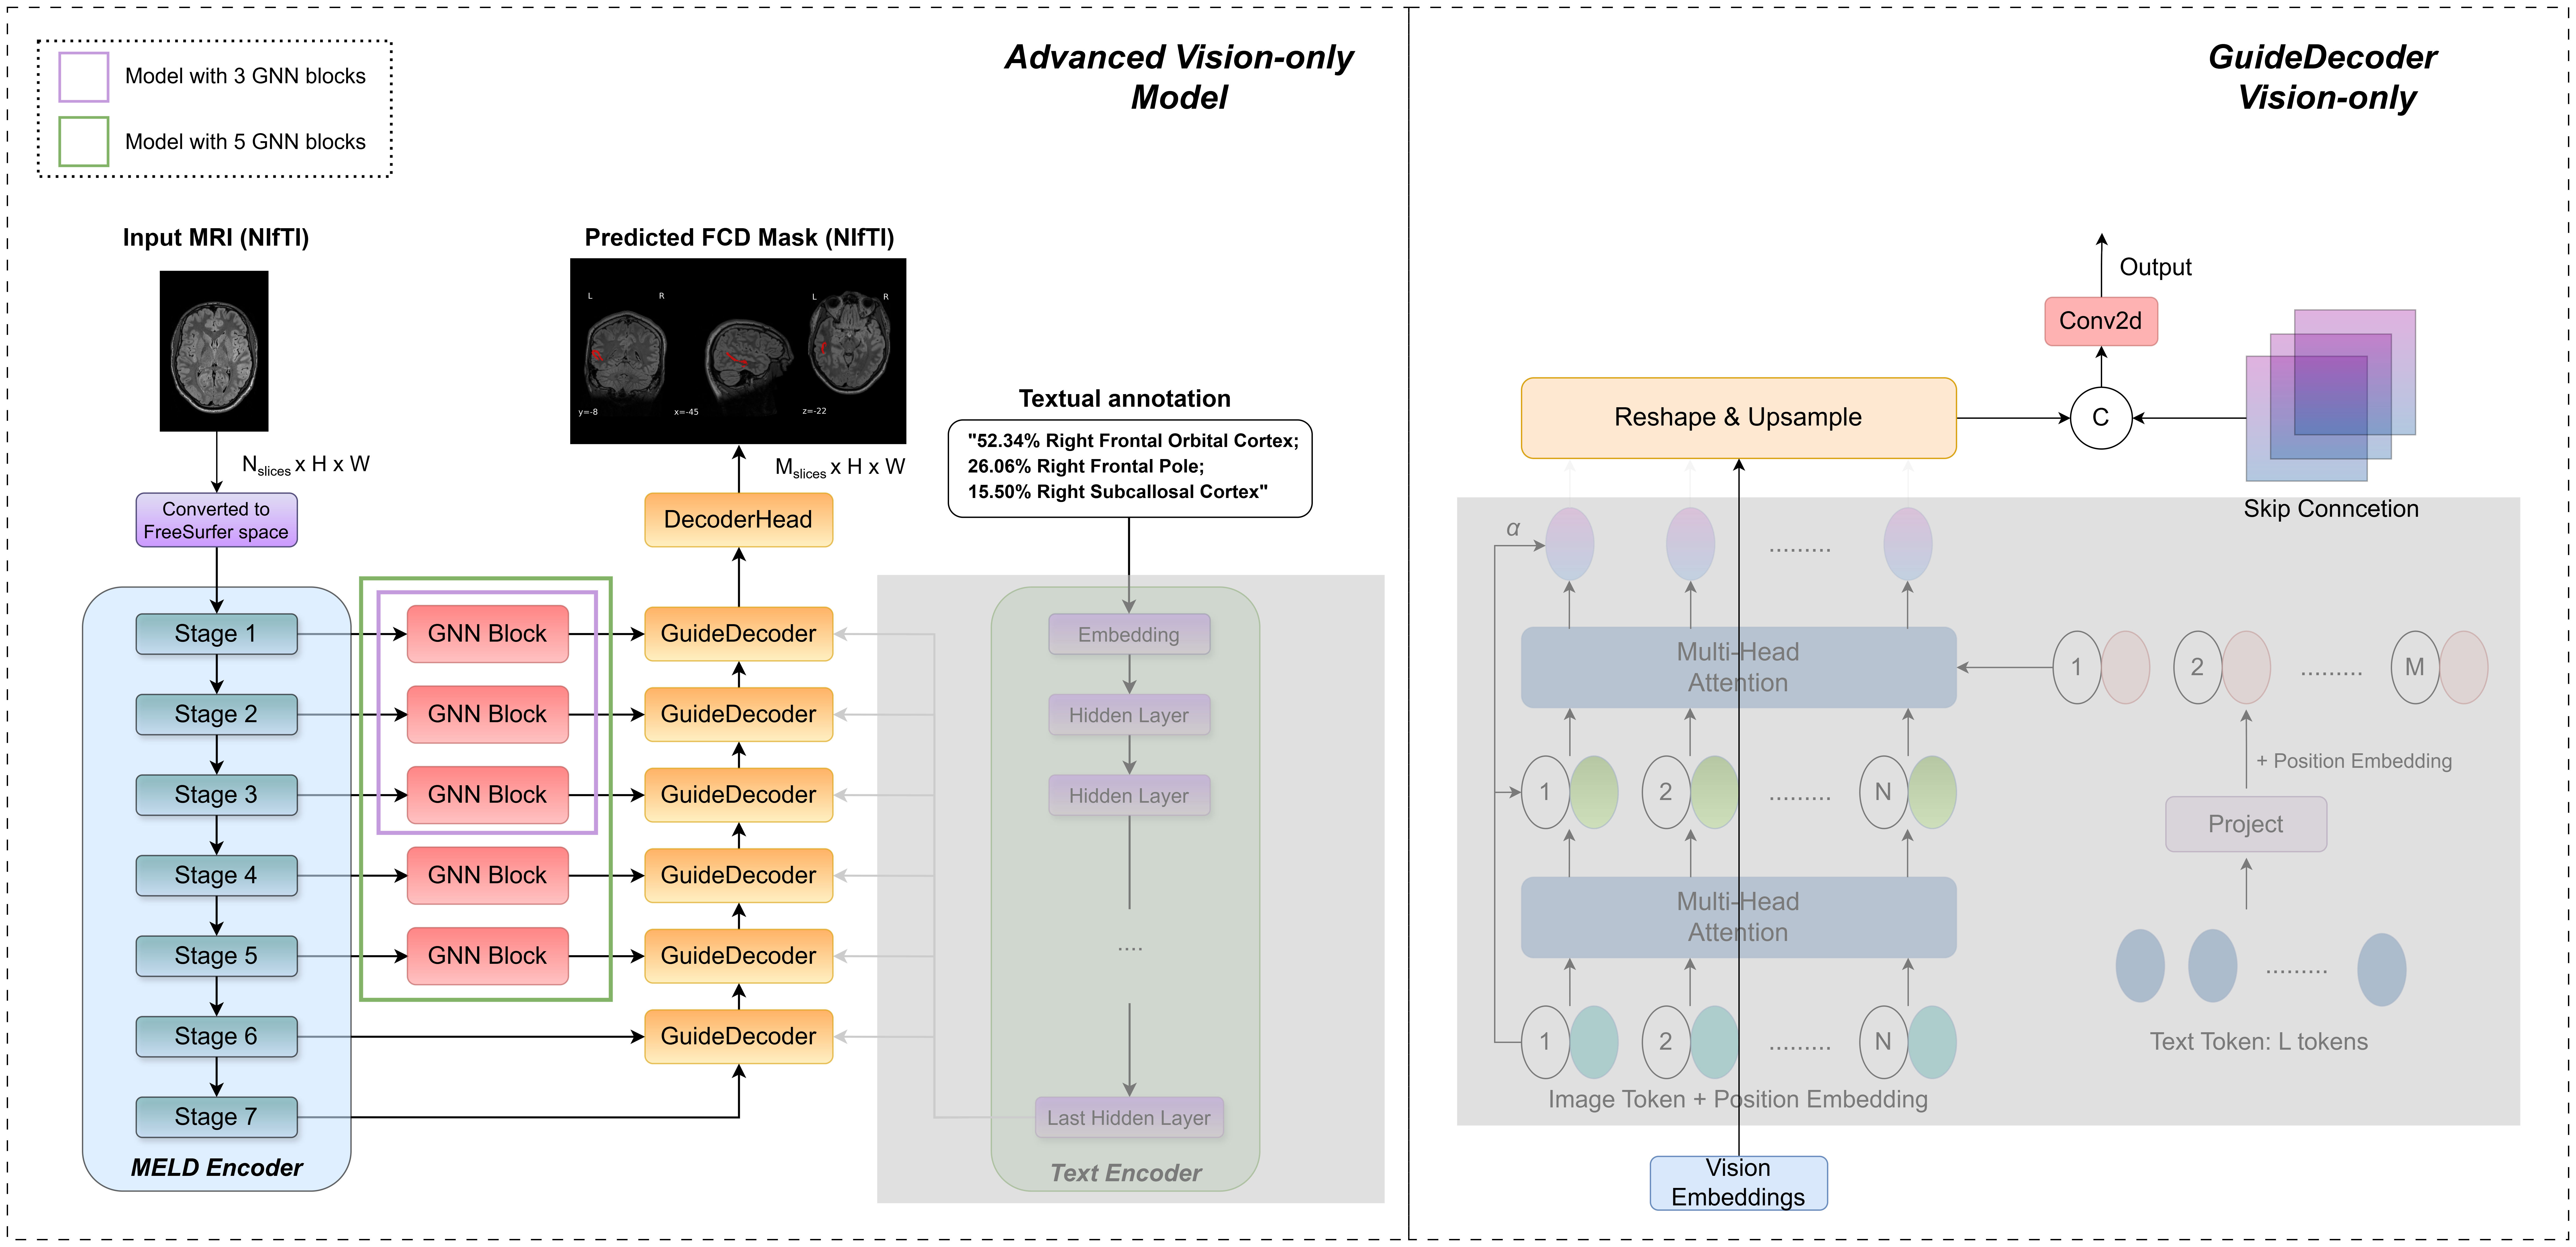
\includegraphics[width=\textwidth]{pictures/AdvancedExp1.png}
    \caption{Architecture of Advanced \texttt{Vision--only}: MELD surface-based features are extracted through a multi-stage GNN encoder (3- or 5-block variants) and passed through a hierarchical GuideDecoder with cross-attention to text embeddings. 
    At each decoder stage, visual features are fused with text embeddings, reshaped, and upsampled through geometry-aware operations, before producing the final segmentation via the DecoderHead. 
    The right panel illustrates the internal structure of the GuideDecoder layer, including self- and cross-attention over text and vision tokens, skip connections, and spatial upsampling.}
    \label{fig:advanced_exp1}
\end{figure}

On the main cohort (Table~\ref{tab:main_cohort_final}), in the \textit{hemisphere + lobe} and \textit{no\_text} settings, the models with GNN blocks indeed detect a larger number of lesions. 
However, in most cases the model without a GNN block exhibits higher values across all primary metrics and clearly dominates in terms of \textit{Specificity}.

The PPV\textsubscript{clusters} metric explicitly indicates that GNN-based models produce substantially more false-positive clusters, which negatively affects the overall prediction quality. Therefore, based on the obtained results, no definitive advantage of information aggregation in sparse graphs can be concluded.
\begin{table}[H]
\tiny
\begin{threeparttable}
\centering
\caption{Median performance on the main cohort (with 95\% confidence intervals).} 
\label{tab:main_cohort_final}
\begin{tabular}{ccccccccc}
\textbf{Model} &
\textbf{Text type} &
\textbf{Deocder type} &
\textbf{Dice} &
\makecell{\textbf{PPV}\\\textbf{pixels}} &
\makecell{\textbf{(mean)} \\\textbf{PPV}\\\textbf{clusters}} & 
\textbf{IoU} & 
\makecell{\textbf{Specificity, \%} \\ (N = 193)}&
\makecell{\textbf{Sensitivity, \%} \\ (N = 259)}\\
\midrule
MELD &
-- &
-- &
\makecell{0.230\\(0.107--0.320)} &
\makecell{0.166\\(0.086--0.220)} &
0.515 &
\makecell{0.130\\(0.057--0.190)} &
\makecell{58.0 (n=112) \\ (51.3--64.8)} &
\makecell{65.6 (n=170) \\ (59.8--71.4)} \\

\hline

\multirow{3}{*}{\makecell[c]{Vision+LM\_mixed}} &
\multirow{3}{*}{\makecell[c]{hemisphere}} &
\makecell{Vision--only \\ with 3 GNN} &
\makecell{\textbf{0.232} \\ (0.141-0.312)} &
\makecell{0.212 \\ (0.146-0.330)} &
\makecell{0.314} &
\makecell{\textbf{0.131} \\ (0.076-0.185)} &
\makecell{8.3 (n=16) \\ (4.7--12.4)} &
\makecell{69.9 (n=181) \\ (64.1--75.3)} \\
% second row
& 
&
\makecell{Vision--only \\ with 5 GNN} &
\makecell{0.211 \\ (0.110--0.320)} &
\makecell{\textbf{0.226} \\ (0.154--0.394)} &
\makecell{0.242} &
\makecell{0.118 \\ (0.058--0.191)} &
\makecell{1.0 (n=2) \\ (0.0--2.6)} &
\makecell{72.2 (n=187) \\ (66.8--77.6)} \\
% third row
& 
&
\makecell{Basic \\ Vision--only} &
\makecell{0.225 \\ (0.131--0.294)} &
\makecell{0.215 \\ (0.137--0.325)} &
\textbf{0.401} &
\makecell{0.127 \\ (0.070--0.172)} &
\makecell{\textbf{88.1 (n=170)} \\ (83.4--92.2)} &
\makecell{\textbf{73.7 (n=191)} \\ (68.3--79.2)} \\

\hline

\multirow{3}{*}{\makecell[c]{Vision+LM\_mixed}} &
\multirow{3}{*}{\makecell[c]{hemisphere \\ + \\ lobe}} &
\makecell{Vision--only \\ with 3 GNN} &
\makecell{0.224 \\ (0.154-0.319)} &
\makecell{0.200 \\ (0.142-0.314)} &
\makecell{0.310} &
\makecell{0.126 \\ (0.083-0.190)} &
\makecell{8.3 (n=16) \\ (4.7--12.4)} &
\makecell{69.5 (n=180) \\ (63.7--74.9)}\\% second row
& 
&
\makecell{Vision--only \\ with 5 GNN} &
\makecell{0.186 \\ (0.119--0.314)} &
\makecell{0.241 \\ (0.158--0.384)} &
\makecell{0.246} &
\makecell{0.103 \\ (0.063--0.186)} &
\makecell{1.0 (n=2) \\ (0.0--2.6)} &
\makecell{\textbf{71.8 (n=186)} \\ (66.4--77.2)} \\
% third row
& 
&
\makecell{Basic \\ Vision--only} &
\makecell{\textbf{0.228} \\ (0.129--0.321)} &
\makecell{\textbf{0.247} \\ (0.180--0.330)} &
\textbf{0.482} &
\makecell{\textbf{0.129} \\ (0.069--0.180)} &
\makecell{\textbf{88.1 (n=170)} \\ (83.4--92.2)} &
\makecell{71.0 (n=184) \\ (65.6--76.4)} \\

\hline

\multirow{3}{*}{\makecell[c]{Vision+LM\_mixed}} &
\multirow{3}{*}{\makecell[c]{no text}} &
\makecell{Vision--only \\ with 3 GNN} &
\makecell{0.212 \\ (0.120-0.311)} &
\makecell{\textbf{0.262} \\ (0.164-0.355)} &
\makecell{0.206} &
\makecell{0.119 \\ (0.064-0.184)} &
\makecell{0.0 (n=0) \\ (0.0--0.0)} &
\makecell{\textbf{72.2 (n=187)} \\ (66.8--77.6)}\\
% second row
& 
&
\makecell{Vision--only \\ with 5 GNN} &
\makecell{0.229 \\ (0.118--0.311)} &
\makecell{0.259 \\ (0.135--0.363)} &
\makecell{0.235} &
\makecell{0.130 \\ (0.063--0.184)} &
\makecell{1.0 (n=2) \\ (0.0--2.6)} &
\makecell{69.5 (n=180) \\ (63.7--74.9)} \\
% third row
& 
&
\makecell{Basic \\ Vision--only} &
\makecell{\textbf{0.249} \\ (0.080--0.296)} &
\makecell{0.192 \\ (0.127--0.289)} &
\textbf{0.443} &
\makecell{\textbf{0.142} \\ (0.042--0.174)} &
\makecell{\textbf{52.3 (n=101)} \\ (45.1--59.1)} &
\makecell{66.0 (n=171) \\ (60.2--71.8)} \\

\bottomrule
\end{tabular}

\vspace{2mm}
\begin{tablenotes}\footnotesize
\item[] \textit{Note.}
\item \textit{Basic Vision--only} denotes the pretrained \texttt{Vision--only} model without GNN blocks; \textit{Vision--only with 3/5 GNN} denotes the pretrained \texttt{Vision--only} model with 3/5 GNN blocks.
\item Dice, IoU, and PPV metrics are computed on patients only (subjects with lesions).
\item All experiments in this table use the \textit{Vision+LM\_mixed} training scheme to obtain results more efficiently.
\end{tablenotes}


\end{threeparttable}
\end{table}

However, on the independent (Bonn) cohort (Tables~\ref{tab:independent_cohort_final}), we observe that for the 
\textit{hemisphere} and \textit{hemisphere + lobe} settings, the model with \textbf{three GNN blocks} achieves the 
highest Dice, IoU, and Sensitivity. 
However, its PPV\textsubscript{clusters} is almost twice as low as that of the baseline without a GNN block, 
indicating a substantially larger number of false-positive clusters. 
This is further reflected in the \textbf{Specificity}, which is approximately three times lower than the baseline and substantially lower compared to the 5-GNN configuration.

These findings suggest that the number of GNN blocks must be selected with caution: deeper aggregation can cause 
feature oversmoothing, which may negatively affect cluster-level precision, as clearly seen in the 5-GNN case. 
In the \textit{no-text} setting, GNN-based models primarily increase the number of detected lesions, but do so at 
the cost of all remaining metrics, indicating reduced prediction quality.

\begin{table}[H]
    \tiny
    \renewcommand{\arraystretch}{1.4}
    \begin{threeparttable}
    \centering
    \caption{Median performance on the independent cohort (with 95\% confidence intervals).} 
    \label{tab:independent_cohort_final}
    \begin{tabular}{ccccccccc}
    \textbf{Model} &
    \textbf{Text type} &
    \textbf{Deocder type} &
    \textbf{Dice} &
    \makecell{\textbf{PPV}\\\textbf{pixels}} &
    \makecell{\textbf{(mean)} \\\textbf{PPV}\\\textbf{clusters}} & 
    \textbf{IoU} & 
    \makecell{\textbf{Specificity, \%} \\ (N = 83)}&
    \makecell{\textbf{Sensitivity, \%} \\ (N = 82)}\\
    \midrule
    MELD &
    -- &
    -- &
    \makecell{0.358\\(0.209--0.465)} &
    \makecell{0.261\\(0.142--0.428)} &
    0.464 &
    \makecell{0.218\\(0.117--0.303)} &
    \makecell{55.4 (n=46) \\ (44.6--66.3)} & 
    \makecell{69.5 (n=57) \\ (59.8--79.3)} \\
    
    \hline
    
    \multirow{3}{*}{\makecell[c]{Vision+LM\_mixed}} &
    \multirow{3}{*}{\makecell[c]{hemisphere}} &
    \makecell{Vision--only \\ with 3 GNN} &
    \makecell{\textbf{0.446} \\ (0.289--0.553)} &
    \makecell{0.404 \\ (0.228--0.605)} &
    \makecell{0.294} &
    \makecell{\textbf{0.288} \\ (0.169--0.382)} &
    \makecell{33.7 (n=28) \\ (24.1--44.6)} &
    \makecell{\textbf{78.0 (n=64)} \\ (68.3--86.6)} \\
    % second row
    &
    &
    \makecell{Vision--only \\ with 5 GNN} &
    \makecell{0.378 \\ (0.274--0.549)} &
    \makecell{\textbf{0.418} \\ (0.237--0.667)} &
    \makecell{0.186} &
    \makecell{0.233 \\ (0.159--0.379)} &
    \makecell{1.2 (n=1) \\ (0.0--3.6)} &
    \makecell{75.6 (n=62) \\ (65.9--84.1)} \\
    % third row
    &
    &
    \makecell{Basic \\ Vision--only} &
    \makecell{0.368 \\ (0.248--0.505)} &
    \makecell{0.406 \\ (0.218--0.596)} &
    \textbf{0.489} &
    \makecell{0.225 \\ (0.141--0.338)} &
    \makecell{\textbf{94.0 (n=78)} \\ (88.0--98.8)} &
    \makecell{74.4 (n=61) \\ (64.6--84.1)} \\
    
    \hline
    \multirow{3}{*}{\makecell[c]{Vision+LM\_mixed}} &
    \multirow{3}{*}{\makecell[c]{hemisphere \\ + \\ lobe}} &
    \makecell{Vision--only \\ with 3 GNN} &
    \makecell{\textbf{0.412} \\ (0.302--0.565)} &
    \makecell{0.388 \\ (0.217--0.567)} &
    \makecell{0.299} &
    \makecell{\textbf{0.260} \\ (0.178--0.394)} &
    \makecell{33.7 (n=28) \\ (24.1--44.6)} &
    \makecell{\textbf{78.0 (n=64)} \\ (68.3--86.6)} \\
    % second row
    &
    &
    \makecell{Vision--only \\ with 5 GNN} &
    \makecell{0.379 \\ (0.259-0.541)} &
    \makecell{0.408 \\ (0.220-0.666)} &
    \makecell{0.188} &
    \makecell{0.233 \\ (0.148-0.371)} &
    \makecell{1.2 (n=1) \\ (0.0--3.6)} &
    \makecell{75.6 (n=62) \\ (65.9--84.1)} \\
    % third row
    &
    &
    \makecell{Basic \\ Vision--only} &
    \makecell{0.400 \\ (0.162--0.507)} &
    \makecell{\textbf{0.462} \\ (0.239--0.672)} &
    \textbf{0.586} &
    \makecell{0.250 \\ (0.088--0.340)} &
    \makecell{\textbf{94.0 (n=78)} \\ (88.0--98.8)} &
    \makecell{74.4 (n=61) \\ (64.6--84.1)} \\
    \hline

    \multirow{3}{*}{\makecell[c]{Vision+LM\_mixed}} &
    \multirow{3}{*}{\makecell[c]{no text}} &
    \makecell{Vision--only \\ with 3 GNN} &
    \makecell{0.299 \\ (0.161-0.431)} &
    \makecell{0.385 \\ (0.193-0.711)} &
    \makecell{0.202} &
    \makecell{0.176 \\ (0.088-0.274)} &
    \makecell{1.2 (n=1) \\ (0.0--3.6)} &
    \makecell{72.0 (n=59) \\ (62.2--81.7)} \\
    % second row
    &
    &
    \makecell{Vision--only \\ with 5 GNN} &
    \makecell{0.342 \\ (0.242-0.464)} &
    \makecell{0.376 \\ (0.215-0.676)} &
    \makecell{0.191} &
    \makecell{0.206 \\ (0.138-0.302)} &
    \makecell{0.0 (n=0) \\ (0.0--0.0)} &
    \makecell{\textbf{74.4 (n=61)} \\ (64.6--84.1)} \\
    % third row
    &
    &
    \makecell{Basic \\ Vision--only} &
    \makecell{\textbf{0.397} \\ (0.138--0.502)} &
    \makecell{\textbf{0.507} \\ (0.151--0.647)} &
    \textbf{0.549} &
    \makecell{\textbf{0.248} \\ (0.074--0.335)} &
    \makecell{\textbf{68.7 (n=57)} \\ (59.0--78.3)} & 
    \makecell{65.9 (n=54) \\ (54.9--75.6)} \\


    \bottomrule
    \end{tabular}
    
    \vspace{2mm}
    \begin{tablenotes}\footnotesize
    \item[] \textit{Note.}
    \item \textit{Basic Vision--only} denotes the pretrained \texttt{Vision--only} model without GNN blocks; \textit{Vision--only with 3/5 GNN} denotes the pretrained \texttt{Vision--only} model with 3/5 GNN blocks.
    \item Dice, IoU, and PPV metrics are computed on patients only (subjects with lesions).
    \item All experiments in this table use the \textit{Vision+LM\_mixed} training scheme to obtain results more efficiently.
    \end{tablenotes}
    \end{threeparttable}

    \end{table}

Overall, the results show that additional message passing can indeed increase sensitivity for sparse graphs by 
capturing more lesion candidates, but this benefit comes with a pronounced increase in false positives. 
Therefore, while deeper aggregation offers potential advantages, it also highlights the need for further refinement 
of GNN-based feature integration to avoid sacrificing precision.

\end{document}